\chapter{Results} \label{chap:results}
\section{\texorpdfstring{\zinvg}{Z(νν)γ} cross section} \label{sec:results_znng_xsec}
Figure~\ref{fig:postfitXS_CR} shows the postfit plots in the control regions corresponding to the cross section likelihood function.
Figure~\ref{fig:postfitXS_SR} shows the postfit distributions in the vertical and horizontal signal regions.
Figure~\ref{fig:postfitXS_combSR} shows the postfit distribution for both signal regions added together, along with the contributions
made by each true \pTgamma\ bin to the various reconstructed \ETgamma\ bins.

\begin{figure}[htbp]
  \begin{center}
    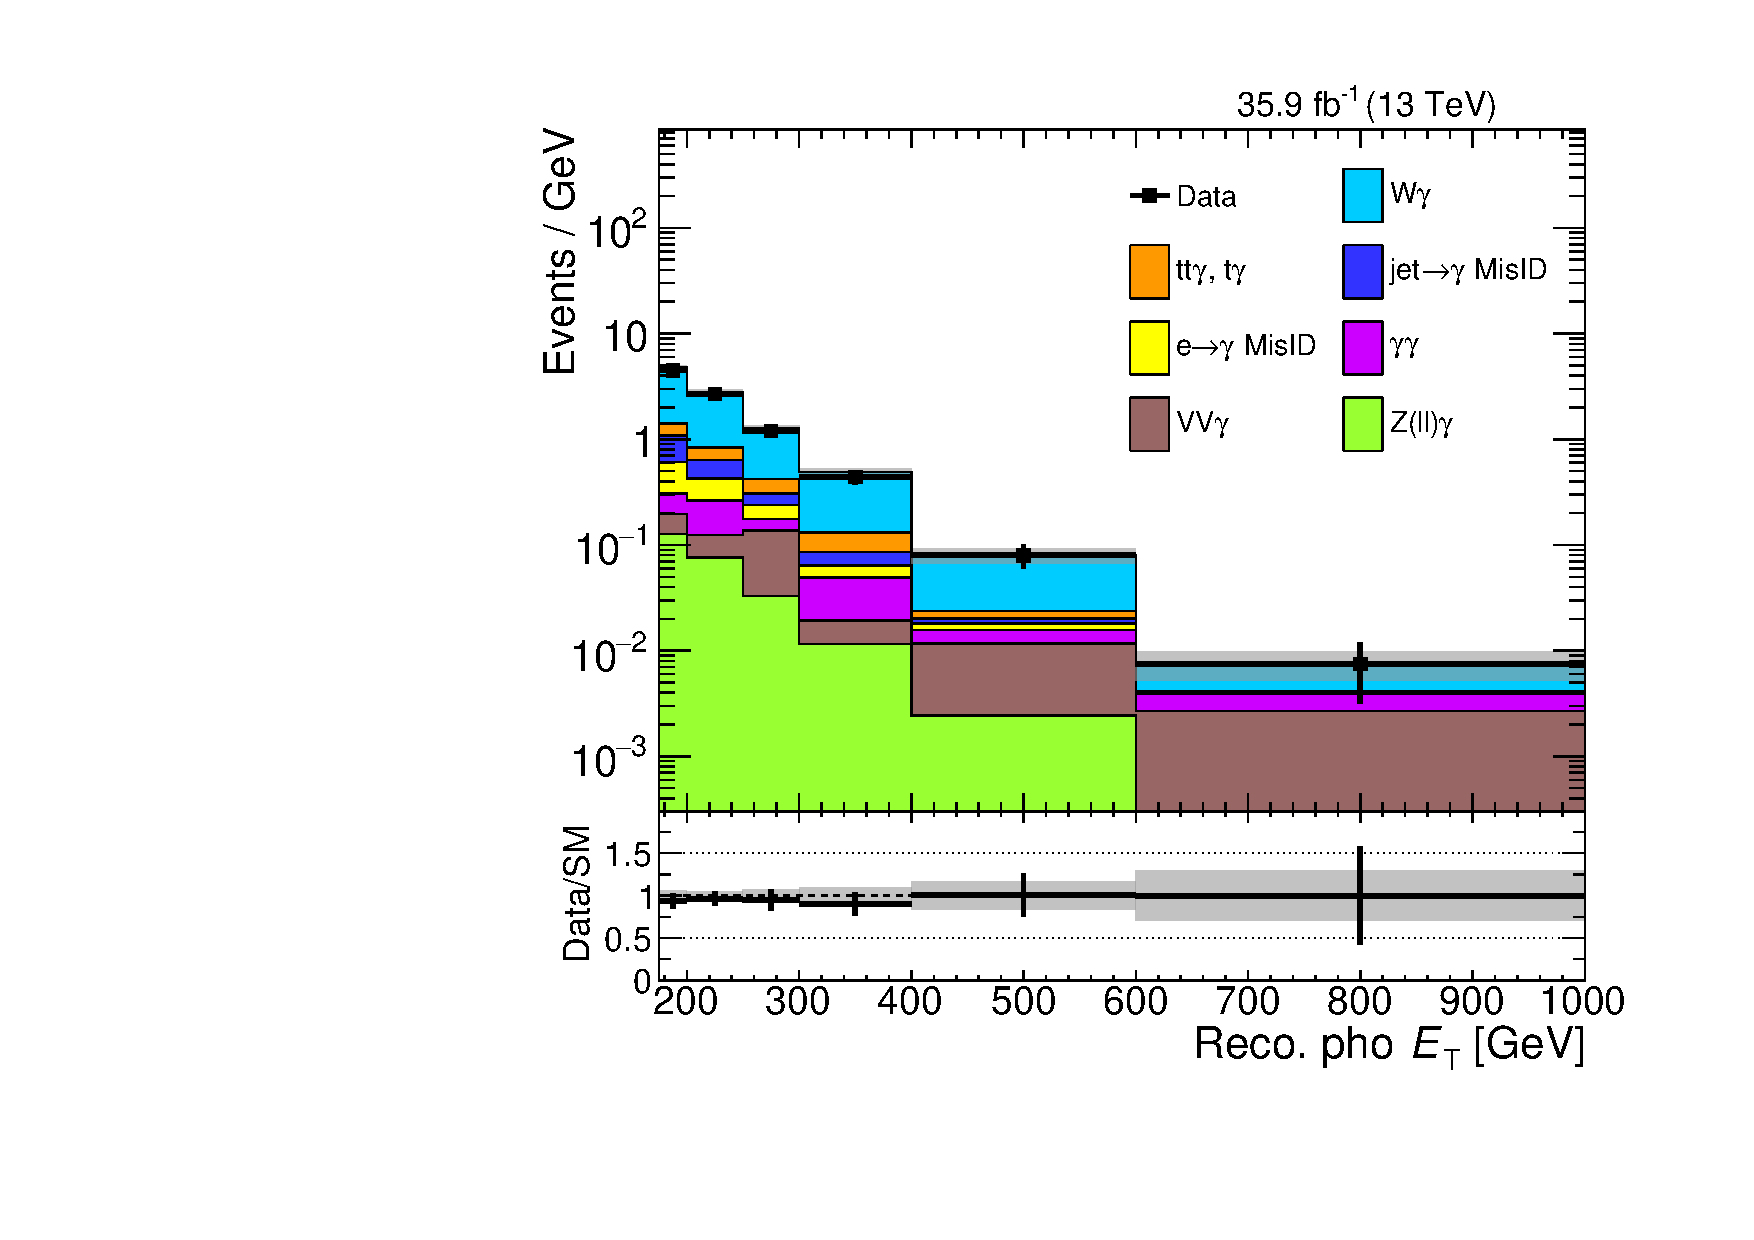
\includegraphics[width=0.45\textwidth]{figures/xsec_results/Postfit/postfit_weng_phoPt.pdf}
    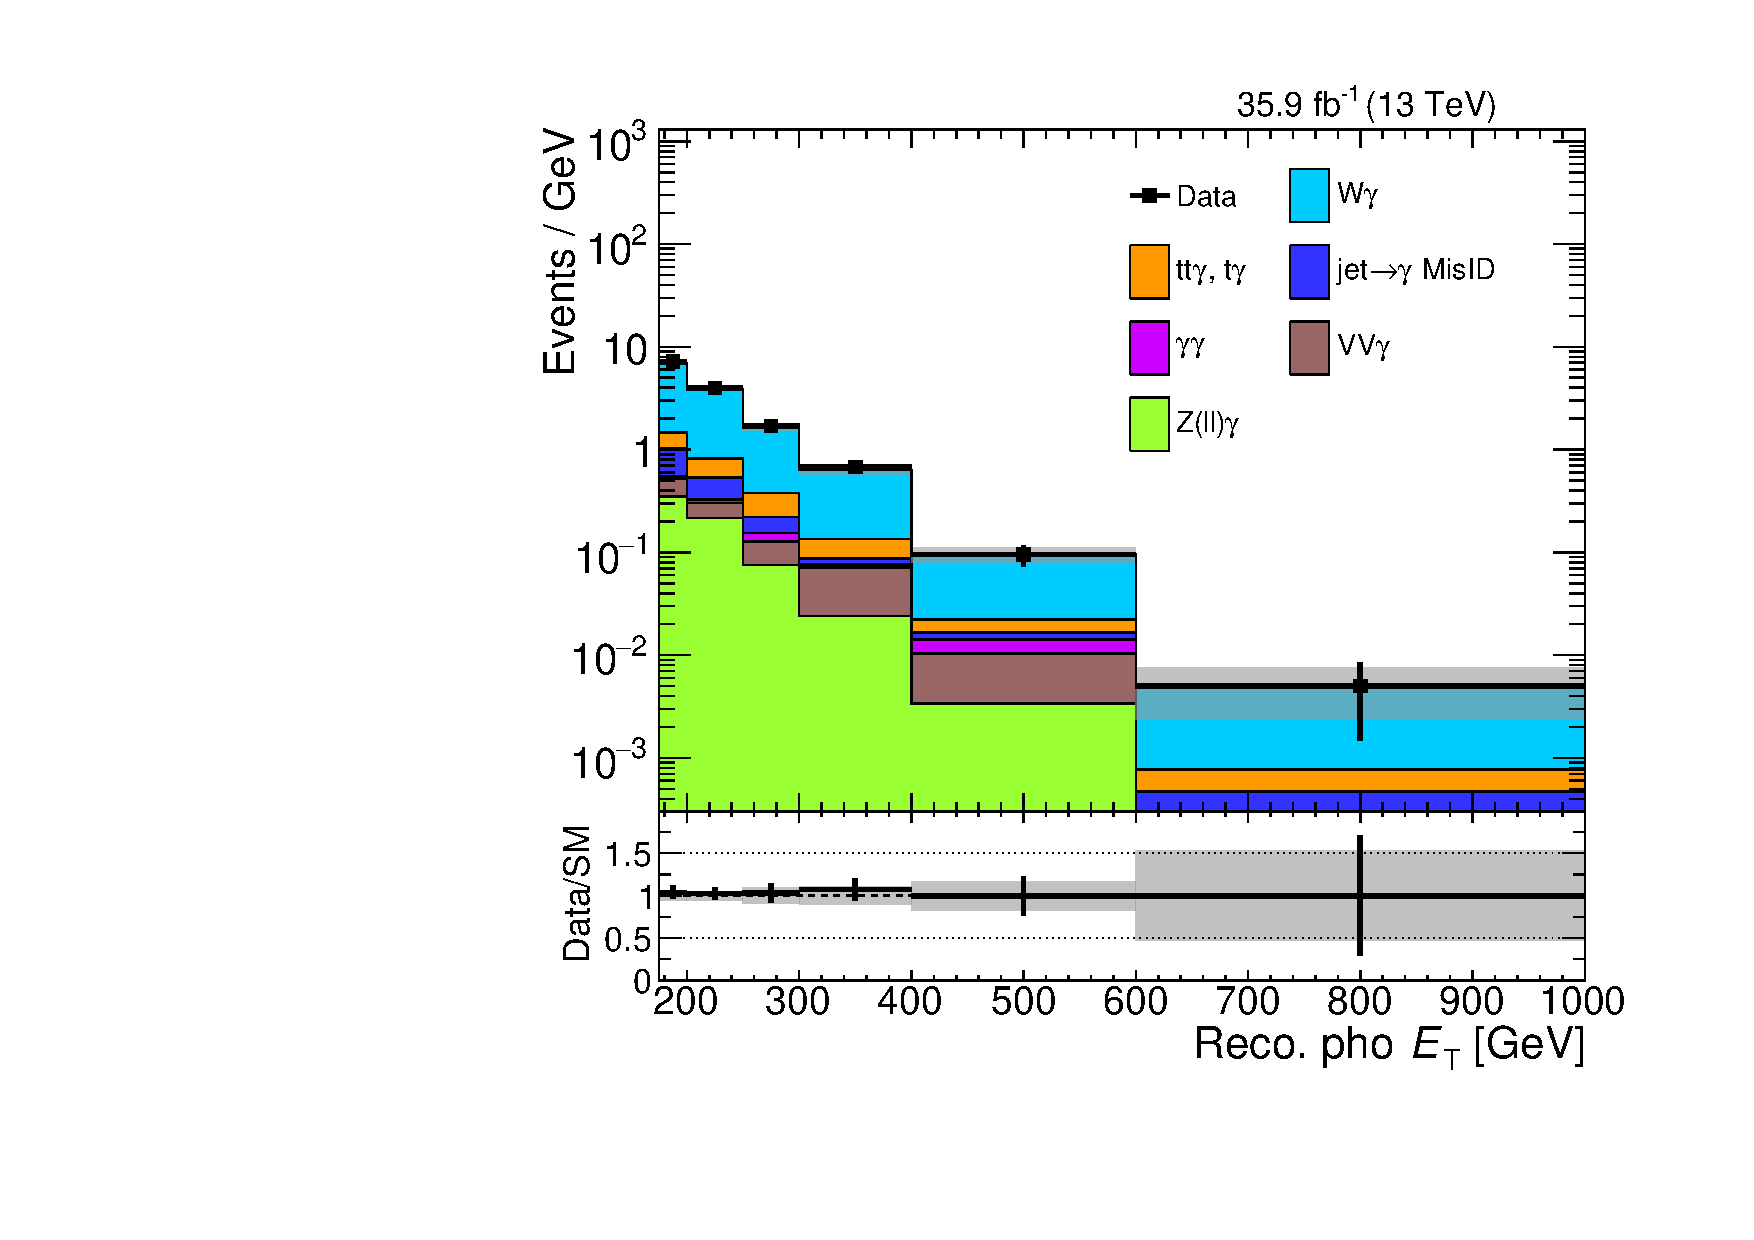
\includegraphics[width=0.45\textwidth]{figures/xsec_results/Postfit/postfit_wmng_phoPt.pdf}
    \caption{
      Control region postfit \ETgamma\ distributions corresponding to the cross section likelihood function:
      \Pe\Pgamma\ (left) and \Pmu\Pgamma\ (right). The last bin includes all events with $\ETgamma > 1000\unit{GeV}$.
    }
    \label{fig:postfitXS_CR}
  \end{center}
\end{figure}

\begin{figure}[htbp]
  \begin{center}
    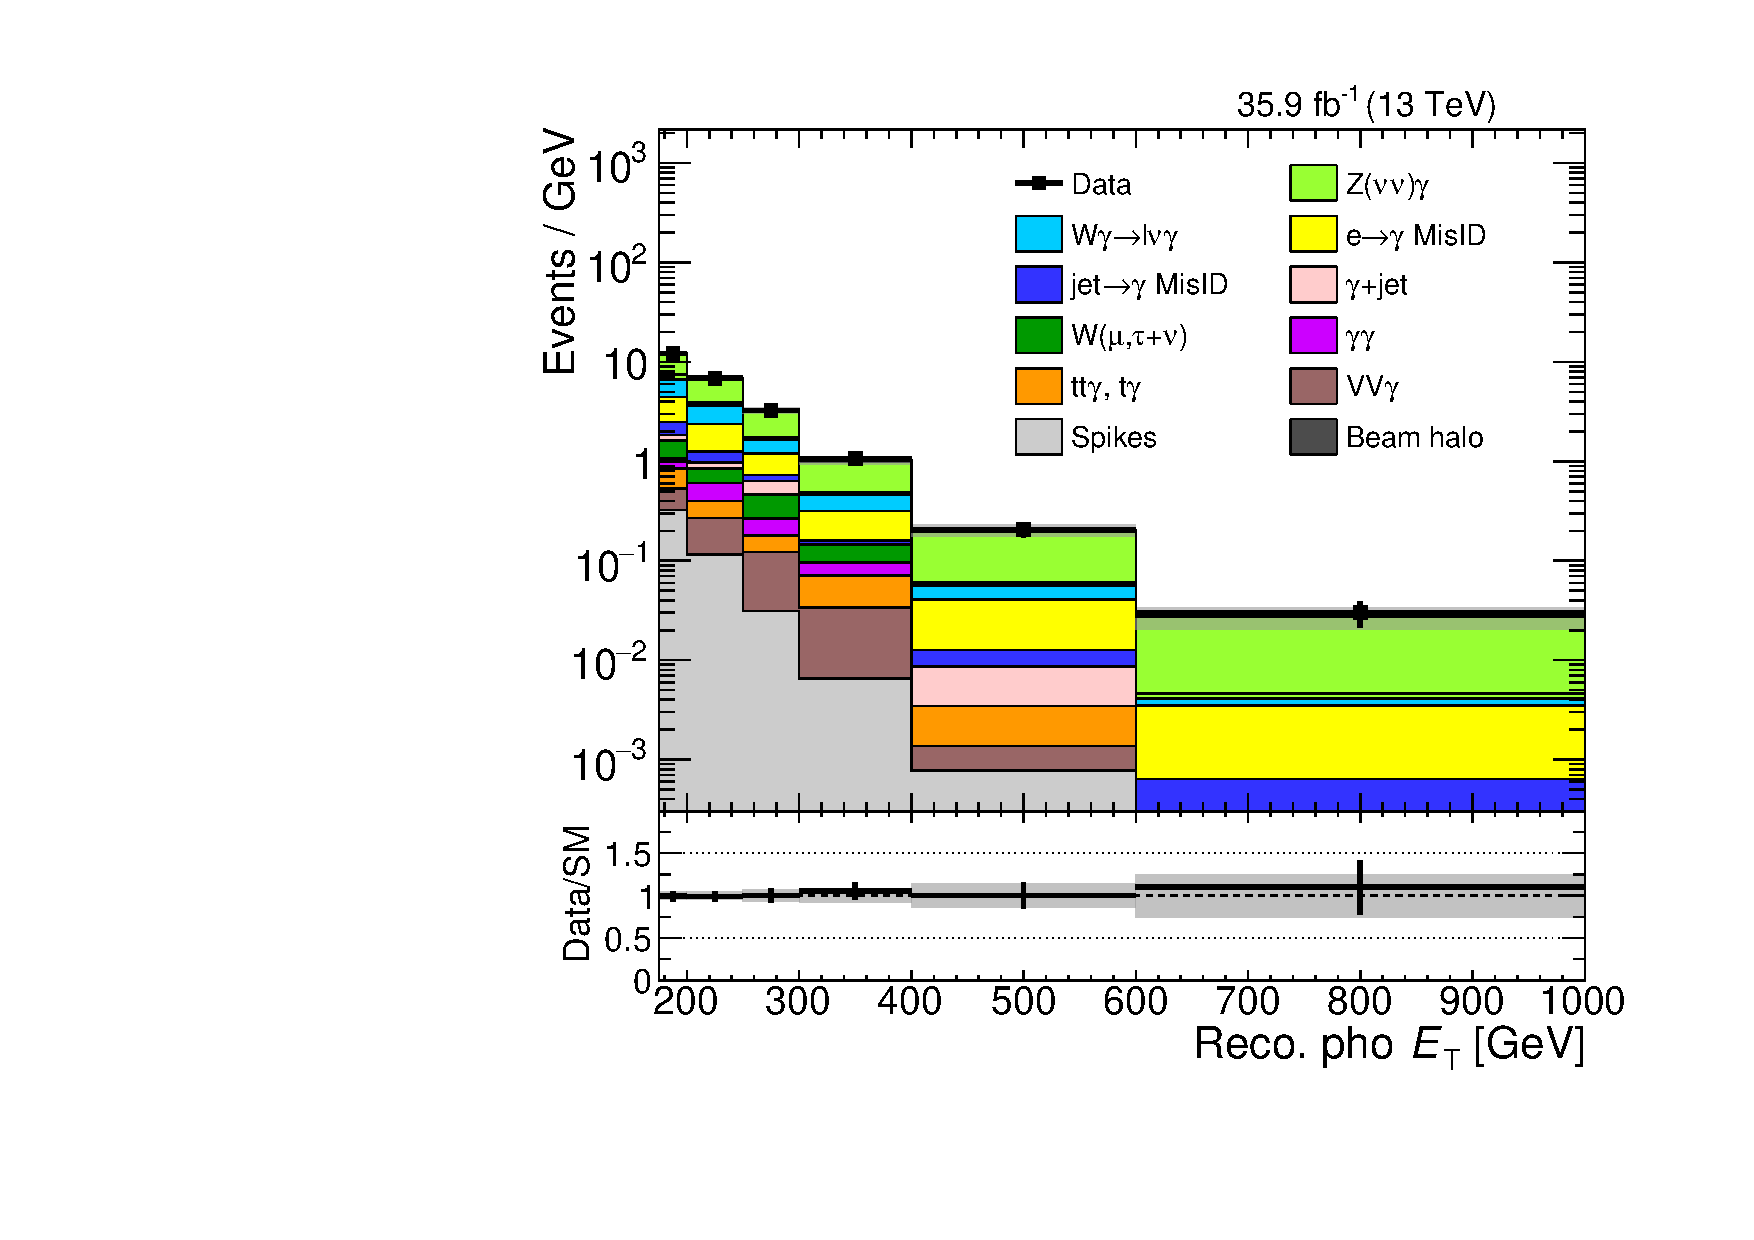
\includegraphics[width=0.45\textwidth]{figures/xsec_results/Postfit/postfit_znng_SA_phoPt.pdf}
    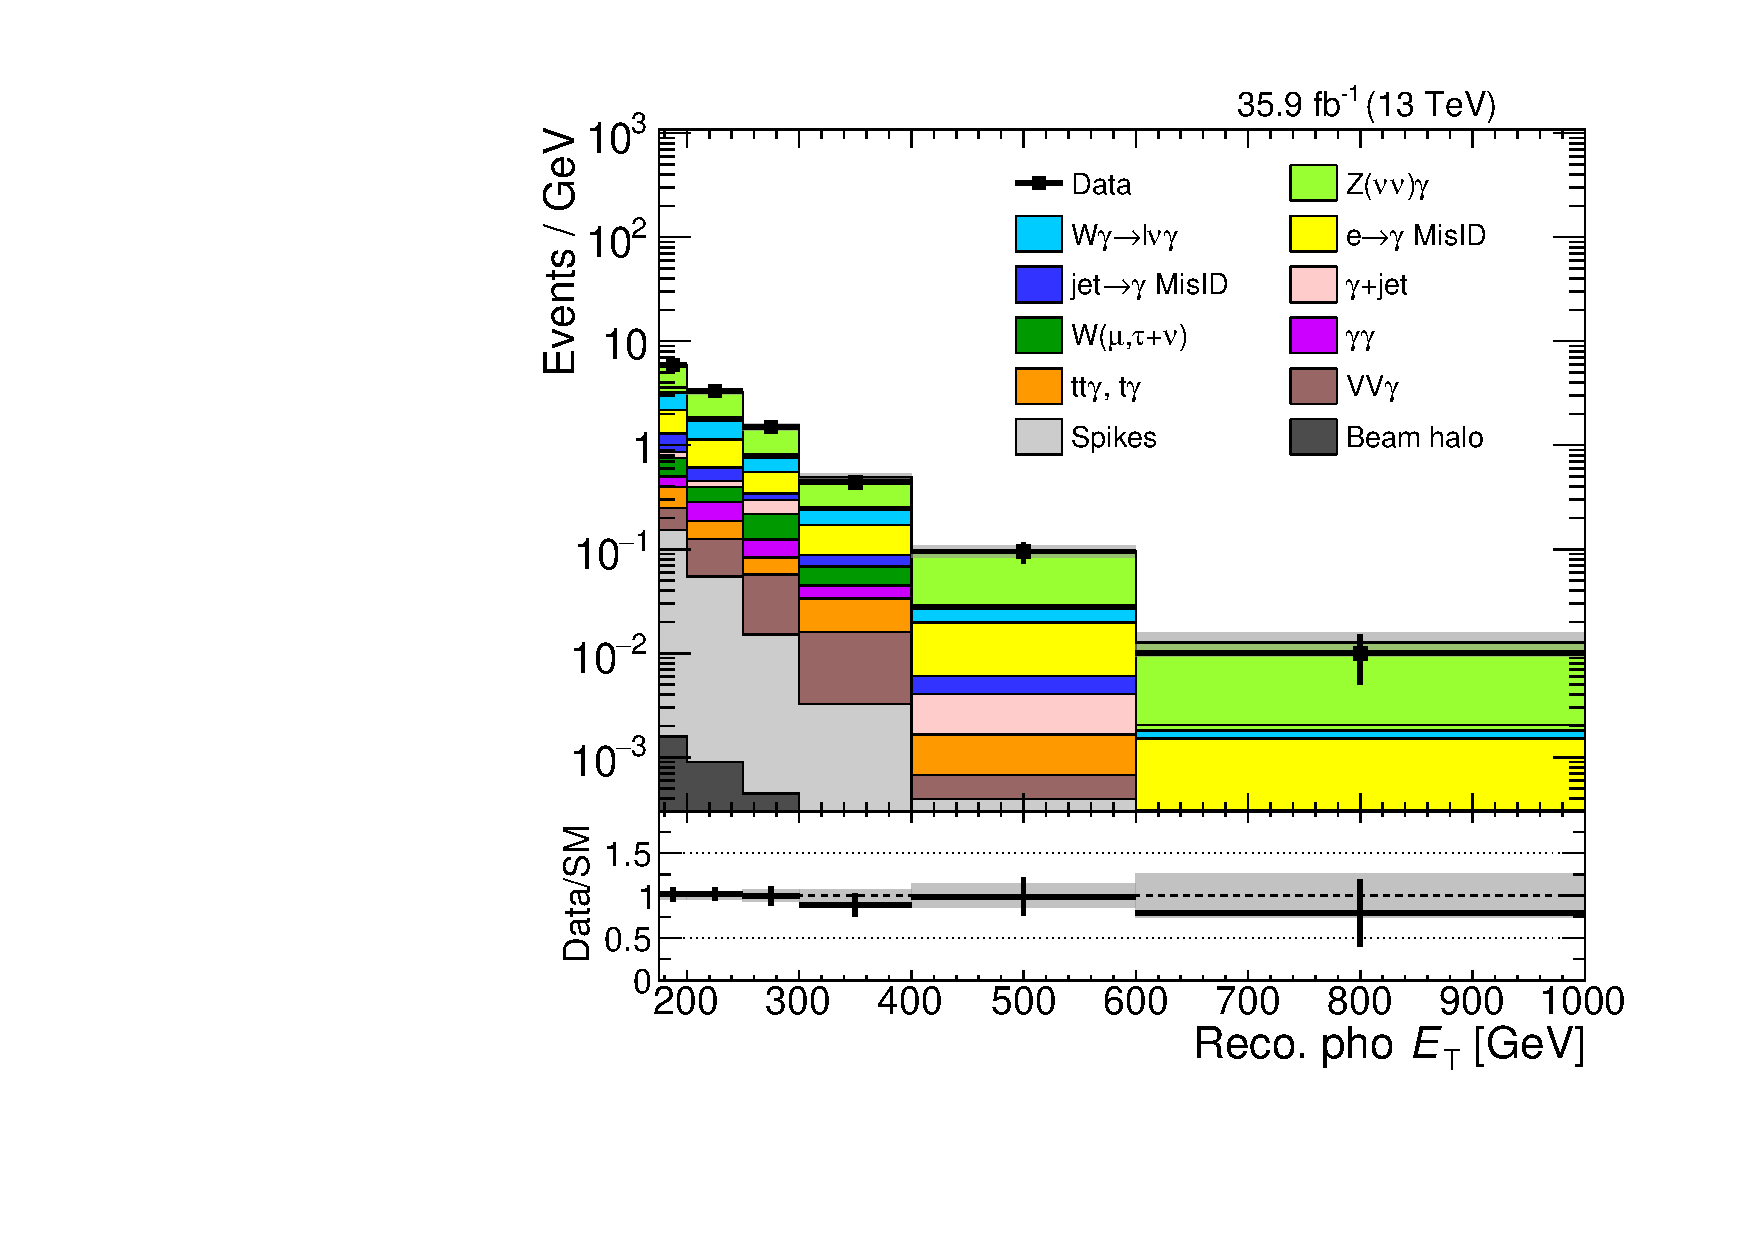
\includegraphics[width=0.45\textwidth]{figures/xsec_results/Postfit/postfit_znng_SB_phoPt.pdf}
    \caption{
      Signal region postfit \ETgamma\ distributions corresponding to the cross section likelihood function:
      vertical region (left) and horizontal region (right).
      The last bin includes all events with $\ETgamma > 1000\unit{GeV}$.
    }
    \label{fig:postfitXS_SR}
  \end{center}
\end{figure}

\begin{figure}[htbp]
  \begin{center}
    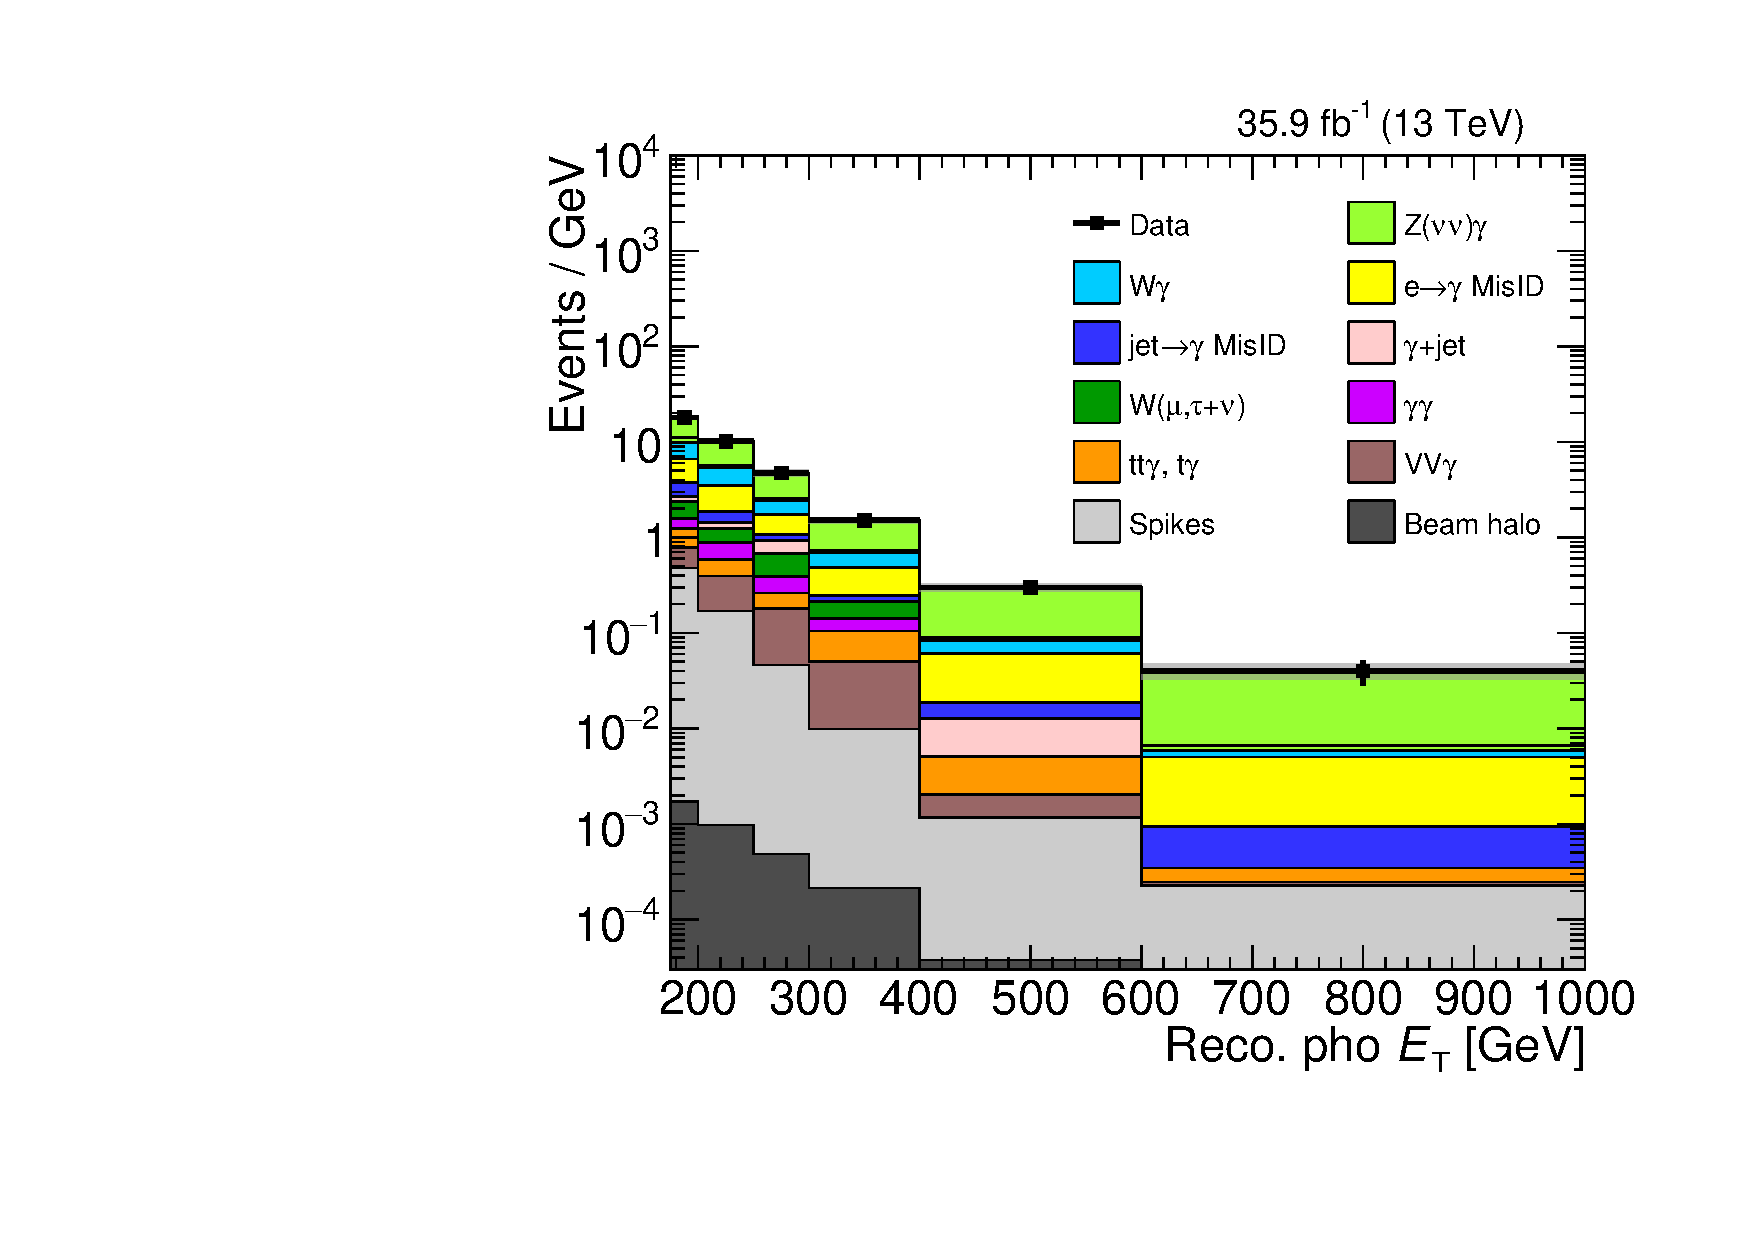
\includegraphics[width=0.45\textwidth]{figures/xsec_results/Postfit/postfit_unfolding_b_phoPt.pdf}
    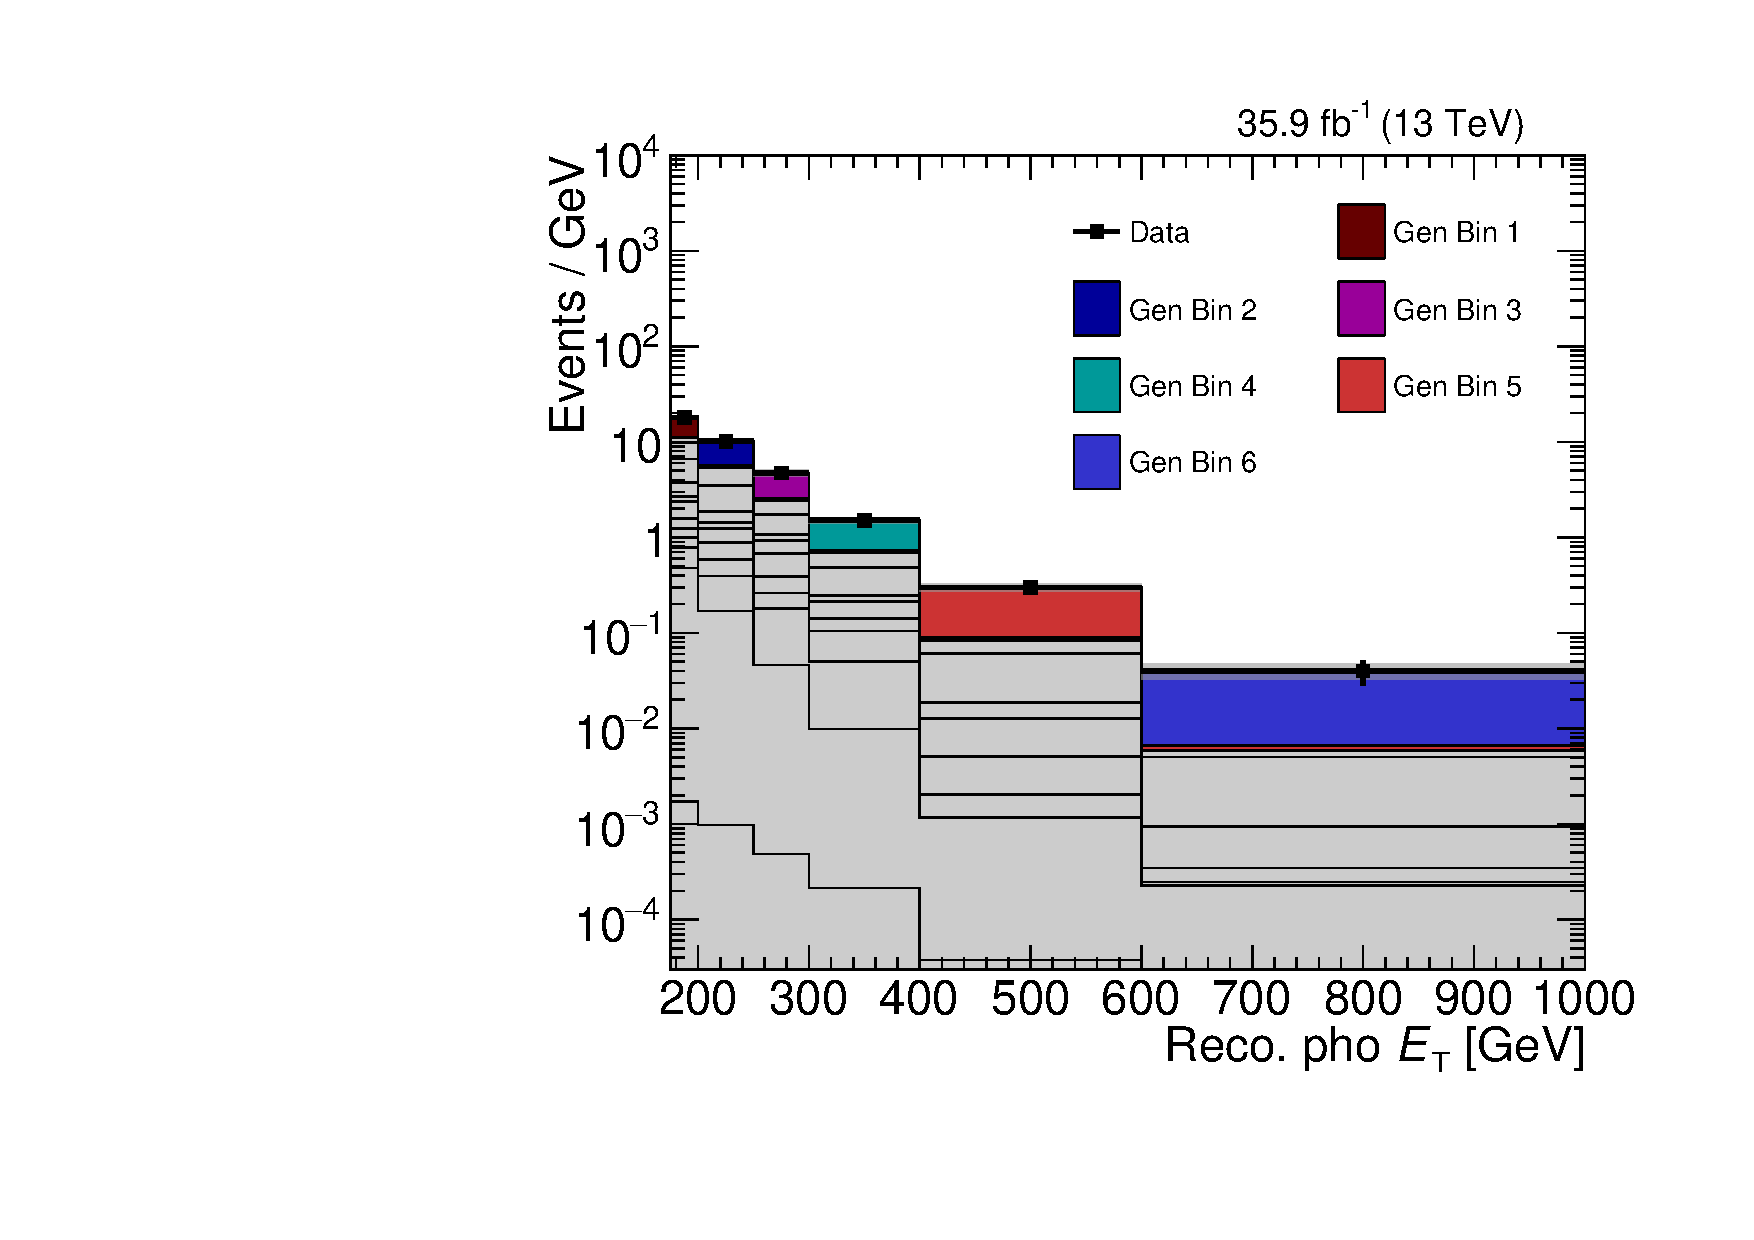
\includegraphics[width=0.45\textwidth]{figures/xsec_results/Postfit/postfit_unfolding_b_genPtAllocation_phoPt.pdf}
    \caption{
      Sum of the postfit reconstructed \ETgamma\ distributions of the two signal regions corresponding to the cross section likelihood function.
      On the left, the separate background contributions are assigned different colors, while \zinvg\ contributions from every bin of true
      \pTgamma\ are assigned the same green color. On the right, all background contributions are assigned the same gray color, while
      contributions from separate \pTgamma\ bins are assigned different colors. The last \ETgamma\ bin includes all events
      with $\ETgamma > 1000\unit{GeV}$.
    }
    \label{fig:postfitXS_combSR}
  \end{center}
\end{figure}

The measured \zinvg\ cross section is listed for each true \pTgamma\ bin in Table~\ref{tab:measured_xsec}, which also lists the uncertainties on the
measurement due to constrained nuisance parameters (systematic uncertainties) and due to the limited size of the observed data set (statistical
uncertainties). For most \pTgamma\ bins, the systematic and statistical uncertainties are of comparable magnitude, but for the highest \pTgamma\ bins
the statistical uncertainty dominates, indicating that the measurement could be significantly refined just by taking additional data (with no change
in methodology).

\begin{table}
\centering
\begin{tabular}{ cccc }
\hline
\pTgamma\ range [GeV] & Cross section [fb] & Syst Unc. [fb] & Stat Unc. [fb] \\
\hline
175-200 & 13.0 & 1.1 (8.7\%) & 1.8 (14\%) \\
200-250 & 14.2 & 0.9 (6.6\%) & 1.6 (11\%) \\
250-300 & 7.3 & 1.1 (15\%) & 1.1 (15\%) \\
300-400 & 5.50 & 0.44 (8.0\%) & 0.92 (17\%) \\
400-600 & 3.31 & 0.15 (4.4\%) & 0.63 (19\%) \\
600-Inf & 1.18 & 0.03 (2.8\%) & 0.36 (30\%) \\
\hline
\end{tabular}
\caption{Measured \zinvg\ cross section in bins of \pTgamma.
The combined uncertainty arising from all constrained nuisance parameters in the likelihood fit is denoted by ``Syst Unc.'', while
uncertainty corresponding to the limited size of the observed data set is denoted by ``Stat Unc.''}
\label{tab:measured_xsec}
\end{table}

% The single-bin uncertainties listed in Table~\ref{tab:measured_xsec} were computed under the assumption that the variations in the measured cross section
% introduced by varying the sources of uncertainty can be examined independently in each bin of \pTgamma. However, varying a source of uncertainty
% can in fact introduce correlated shifts in several cross section bins simultaneously. These correlations are encapsulated by
% the covariance matrix given in Table~\ref{tab:covariance}. This matrix and the corresponding correlation matrix are illustrated in Fig.~\ref{fig:covariance}.
% As that figure shows, the six cross section estimates are largely uncorrelated, with no more than a 20\% correlation between any two
% bins, so to a first approximation the independence assumption of Table~\ref{tab:measured_xsec} is not grossly invalid.

The theoretical SM prediction, as computed in MATRIX to NNLO in $\alpha_\mathrm{S}$, is listed for each true \pTgamma\ bin in Table~\ref{tab:matrix_xsec}, which
also lists the uncertainties on the prediction due to the choice of renormalization and factorization scales (scale uncertainty). Figure~\ref{fig:measvsmat}
compares the measured cross section to the MATRIX predictions.
The two generally agree to within the statistical errors of the measurement, except in the highest \pTgamma\ bins: the difference
between the measured and predicted cross section in the 400-600\unit{GeV} bin is 1.6 times the statistical error on the measurement, and the difference
for the 600-Inf bin is 1.8 times the statistical error. The \zinvg\ process contributes an estimated 13.6 events to the observed 16 events in the 600-Inf bin.
Under the hypothesis that the MATRIX prediction is true, the probability of detecting at least 14 \zinvg\ events
in the 600-Inf bin is about 1\%\footnote{Assuming that \zinvg\ events with true $\pTgamma < 600\unit{GeV}$ contribute negligibly many observed events to this bin
on average (as indicated by the response matrix, Tab.~\ref{tab:response_matrix_values}), and that \zinvg\ events with true $\pTgamma > 600\unit{GeV}$ are produced via a
Poisson process with mean $\sigma_\mathrm{MATRIX}*L = 19.7$ and each such event is detected with probability 0.35 (estimated in MC).}.
This falls far short of the standard ``$5\sigma$'' (about 0.00003\%) criterion for rejecting the SM and claiming discovery of new physics, in particular
since the look-elsewhere effect~\cite{ref:08-AOAS163} is not being accounted for and also since no specific BSM model is being compared here.
However, it does indicate a notable tension with the MATRIX NNLO predictions that should be kept in mind in future studies.

\begin{table}
\centering
\begin{tabular}{ ccc }
\hline
\pTgamma\ range [GeV] & Cross section [fb] & Scale Unc. [fb] \\
\hline
175-200 & 10.53 & 0.18 (1.7\%) \\
200-250 & 12.98 & 0.21 (1.7\%) \\
250-300 & 6.30 & 0.15 (2.4\%) \\
300-400 & 5.01 & 0.14 (2.9\%) \\
400-600 & 2.283 & 0.073 (3.2\%) \\
600-Inf & 0.549 & 0.022 (4.0\%) \\
\hline
\end{tabular}
\caption{SM \zinvg\ cross section in bins of \pTgamma, as computed by the MATRIX generator to NNLO in QCD.
The uncertainty corresponding to the choice of renormalization and factorization scales is denoted by ``Scale Unc.''
The number of generated events was sufficient to render the MC statistical uncertainty negligible in comparison.}
\label{tab:matrix_xsec}
\end{table}

\begin{figure}[htbp]
  \begin{center}
    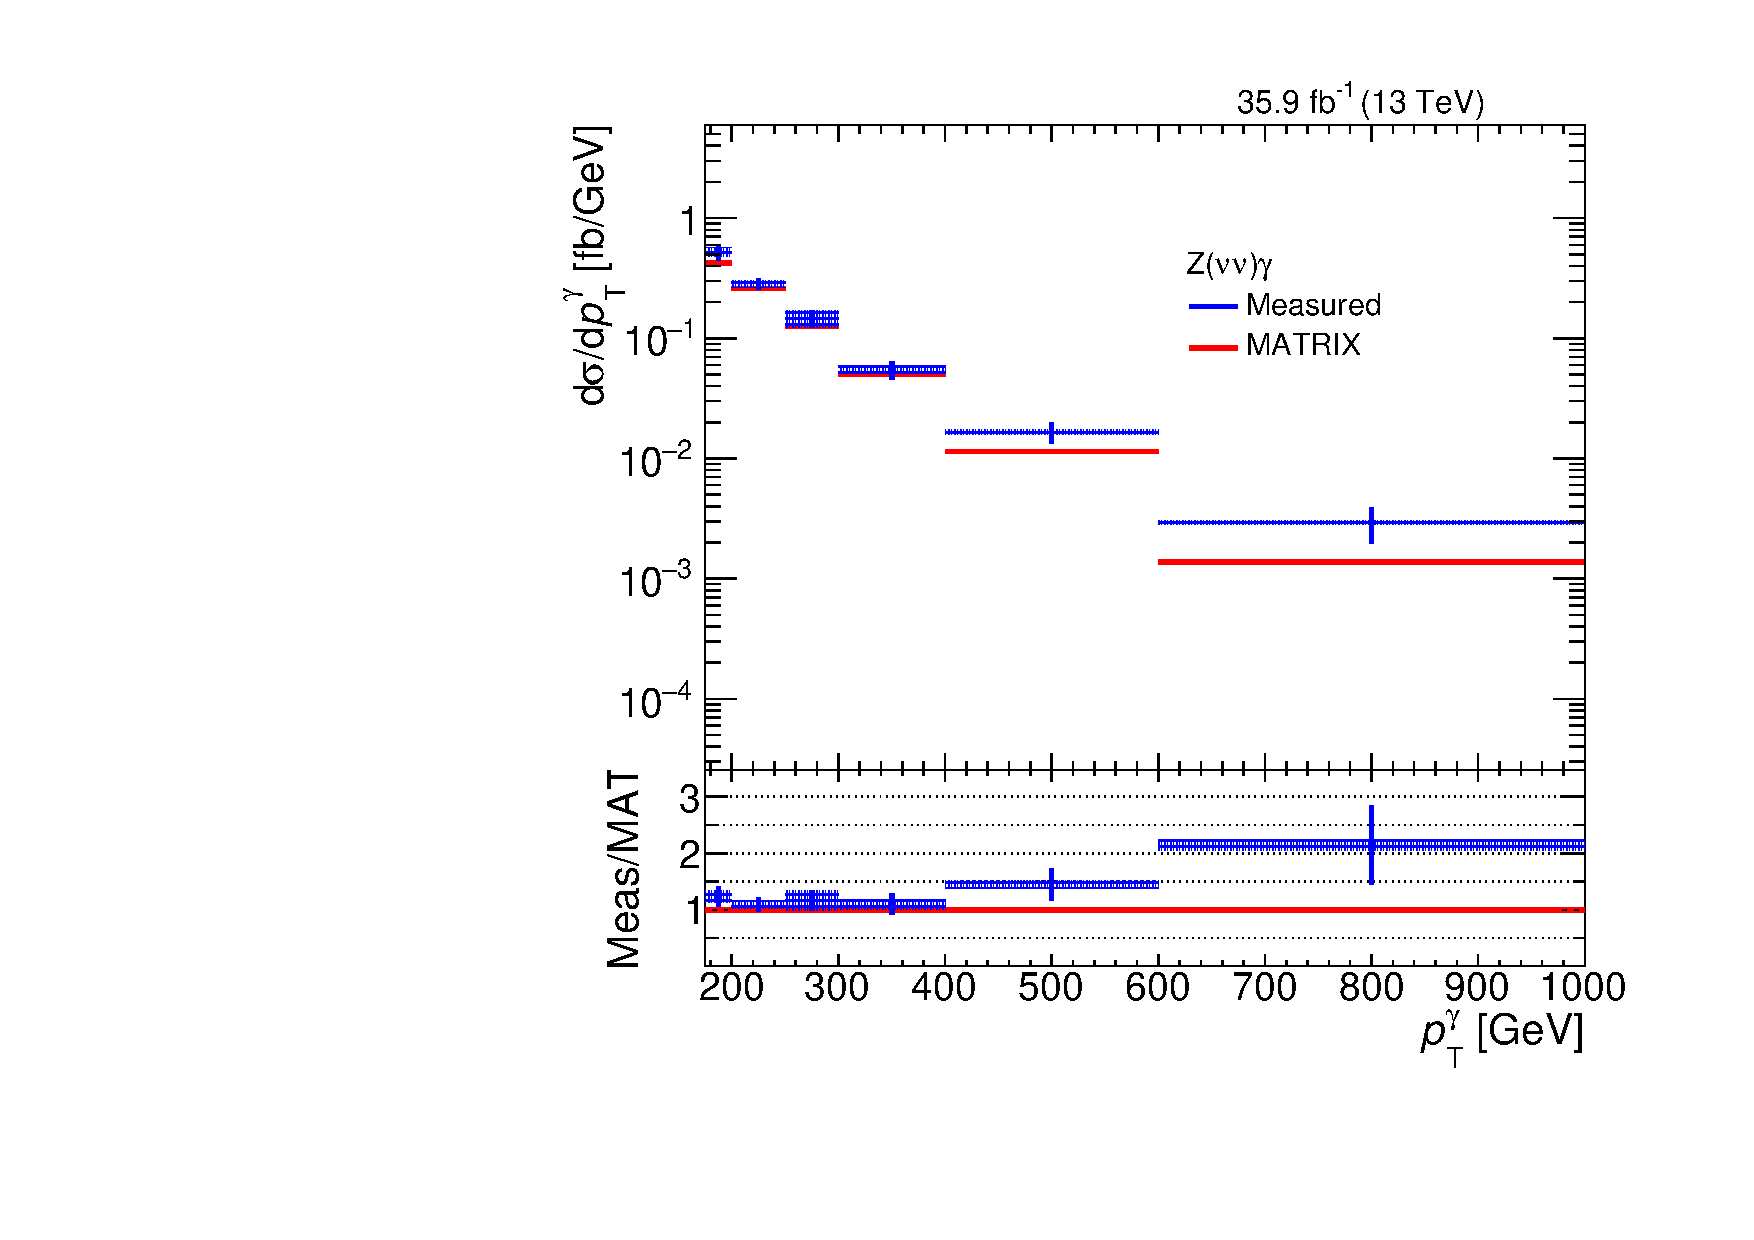
\includegraphics[width=0.75\textwidth]{figures/ZNuNuG_measured_vs_MATRIX.pdf}
    \caption{
      The measured \zinvg\ cross section (blue) compared to the MATRIX NNLO prediction (red). The vertical bars and hatched bands
      on the measured cross section correspond to the statistical and systematic uncertainties, respectively. The scale uncertainty
      on the MATRIX cross section is too small to be seen on this plot. The last bin includes all events with $\pTgamma > 1000\unit{GeV}$.
    }
    \label{fig:measvsmat}
  \end{center}
\end{figure}

\section{DM simplified model limits} \label{sec:results_DM}
Figure~\ref{fig:postfitDM_CR} shows the postfit plots in the control regions corresponding to the DM and ADD likelihood function (with
BSM signal strength fixed to zero\footnote{For nonzero values of the BSM signal strength, the plots depend on a specific choice of BSM model
and parameters. Fixing the signal strength to zero gives a ``model-independent'' perspective on the SM backgrounds,
and essentially illustrates what the estimated backgrounds look like if BSM physics makes imperceptibly
small contributions to observed event yields.}).
Figure~\ref{fig:postfitDM_SR} shows the postfit background distributions in the vertical and horizontal signal regions.
Figure~\ref{fig:2d_mm} shows $\mu_{95}$ in the \mmed--\mdm\ plane for the  vector and
axial-vector mediator scenarios, based on the NLO DM simplified model samples. The solid red curves are the
contours of expected $\mu_{95} = 1$. The DM simplified model hypothesis is excluded at 95\% CL or above in the region with $\mu_{95} < 1$.
For both vector and axial-vector mediators, mediator masses of up to 950\unit{GeV} (observed), 1150\unit{GeV} (expected) are excluded
for small \mdm\ values.
% Figure~\ref{fig:pullsDM} shows how various nuisance parameters are constrained and shifted as
% a result of the fit. None of the parameters are significantly constrained or shifted by the fit.
% Figure~\ref{fig:impacts1} shows
% the impacts of various nuisances parameters on the 95\% CL upper limit of the BSM signal strength for the DM simplified model,
% with a vector mediator of mass $\mmed = 1000\unit{GeV}$ and a dark matter particle of mass $\mdm = 1\unit{GeV}$.

\begin{figure}[htbp]
  \begin{center}
    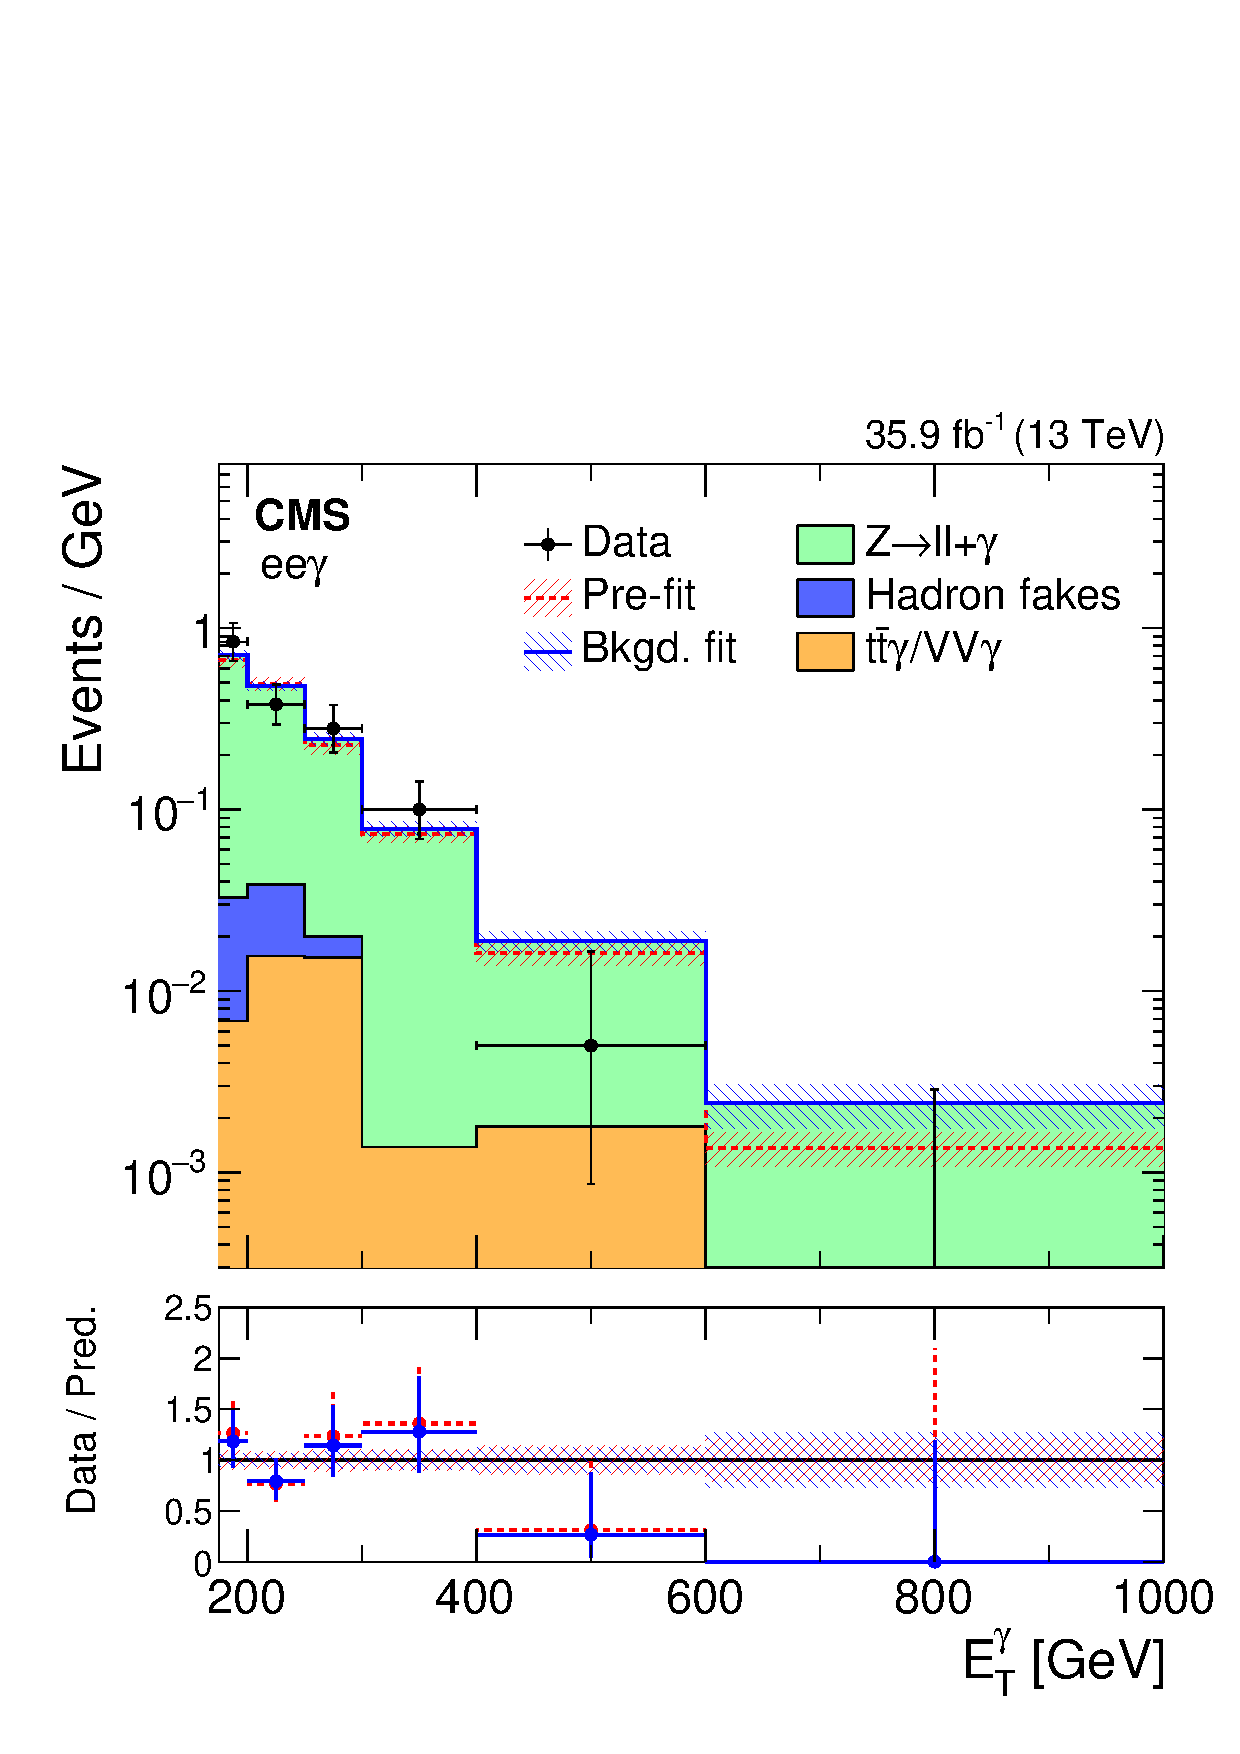
\includegraphics[width=0.45\textwidth]{figures/exo16053/Figure_005-a.pdf}
    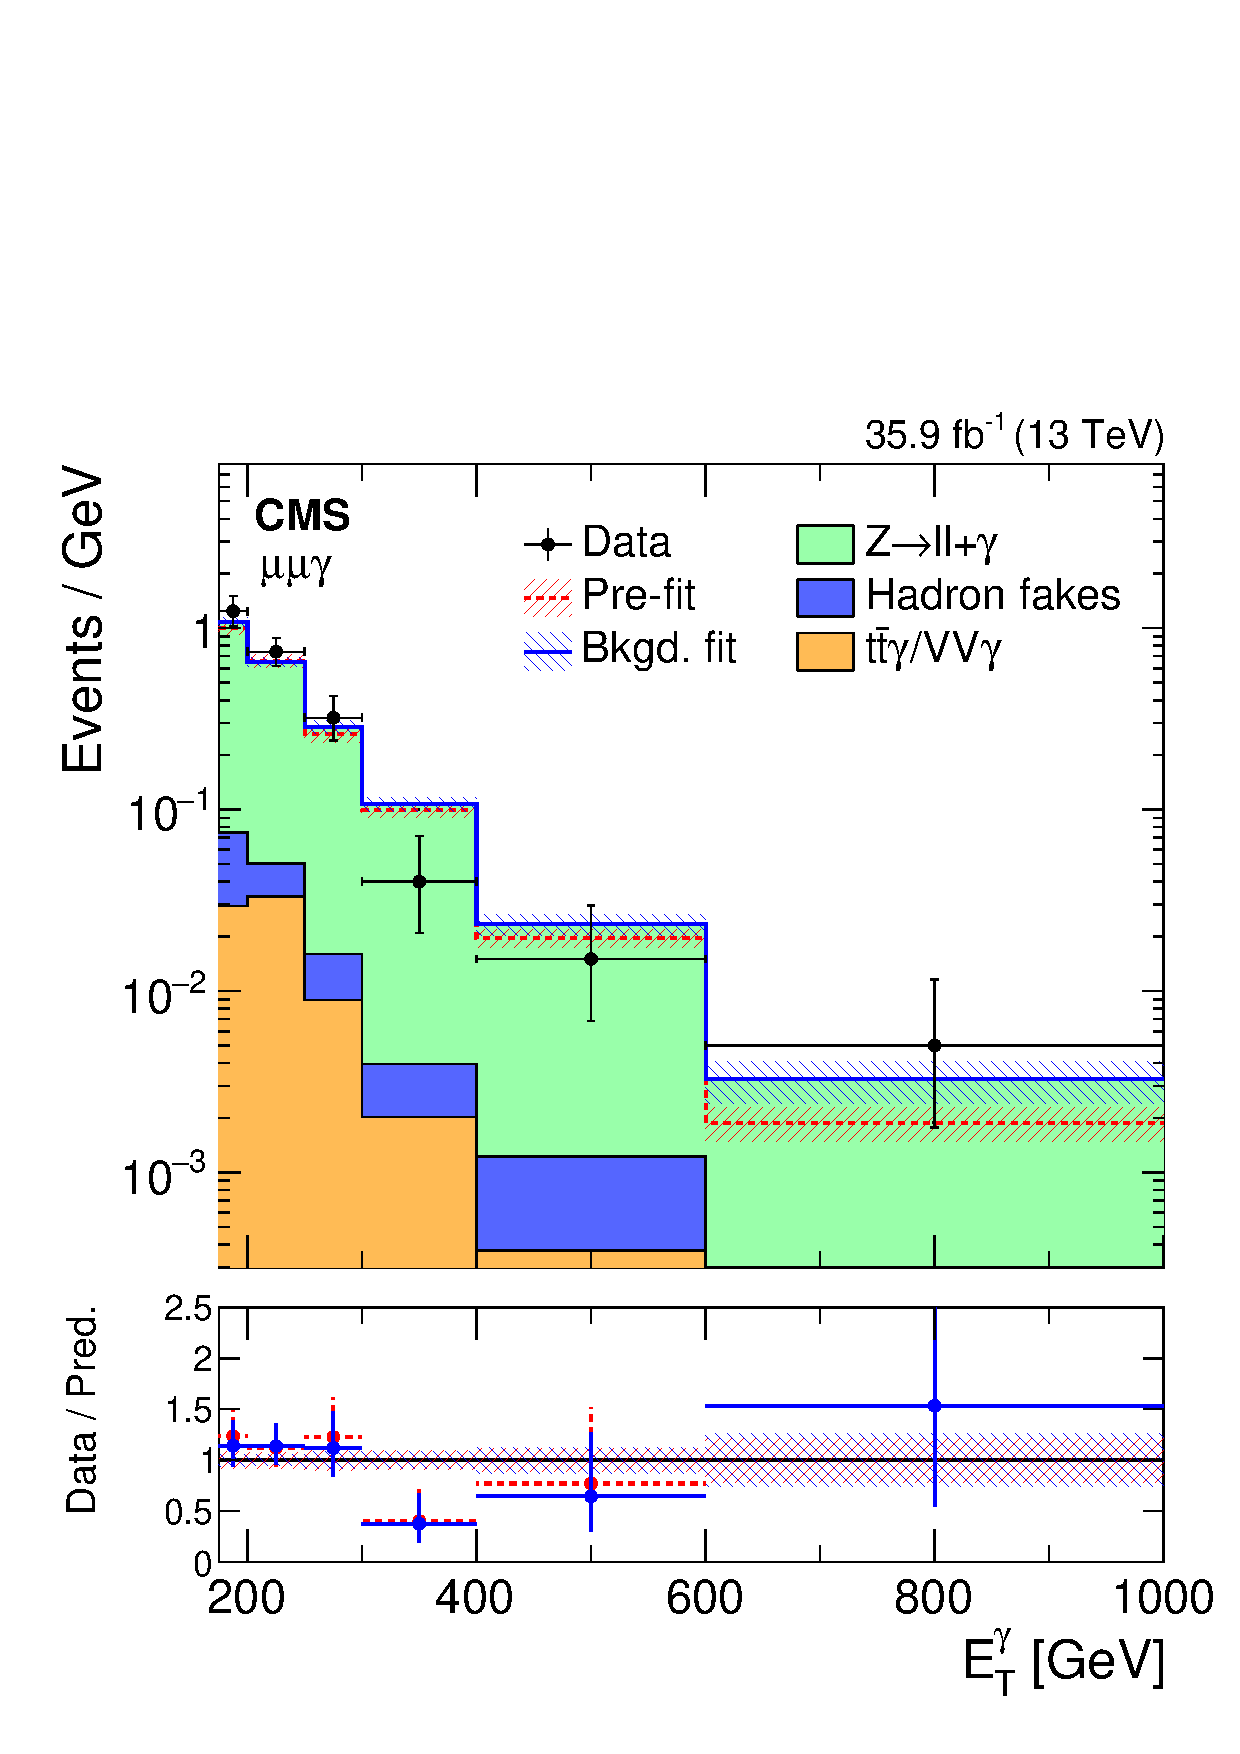
\includegraphics[width=0.45\textwidth]{figures/exo16053/Figure_005-b.pdf}
    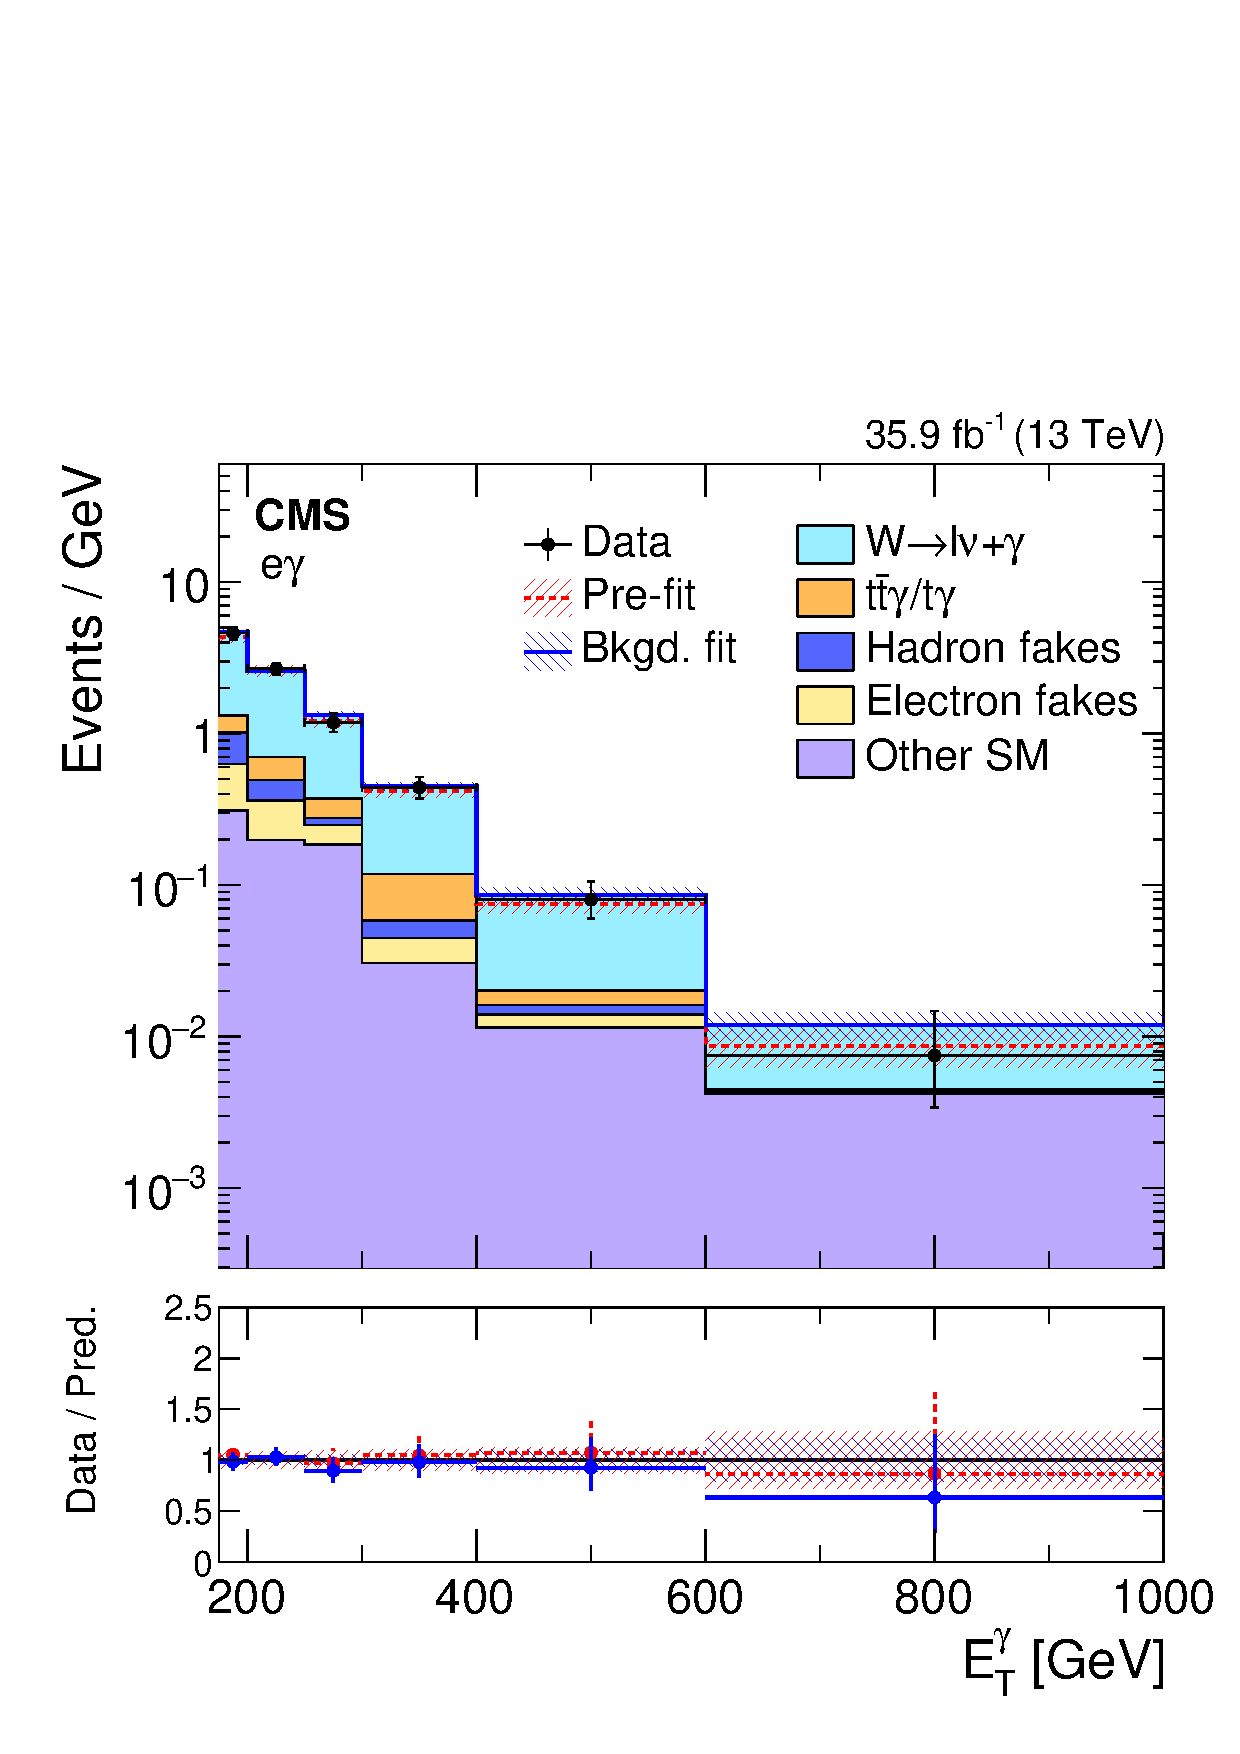
\includegraphics[width=0.45\textwidth]{figures/exo16053/Figure_005-c.pdf}
    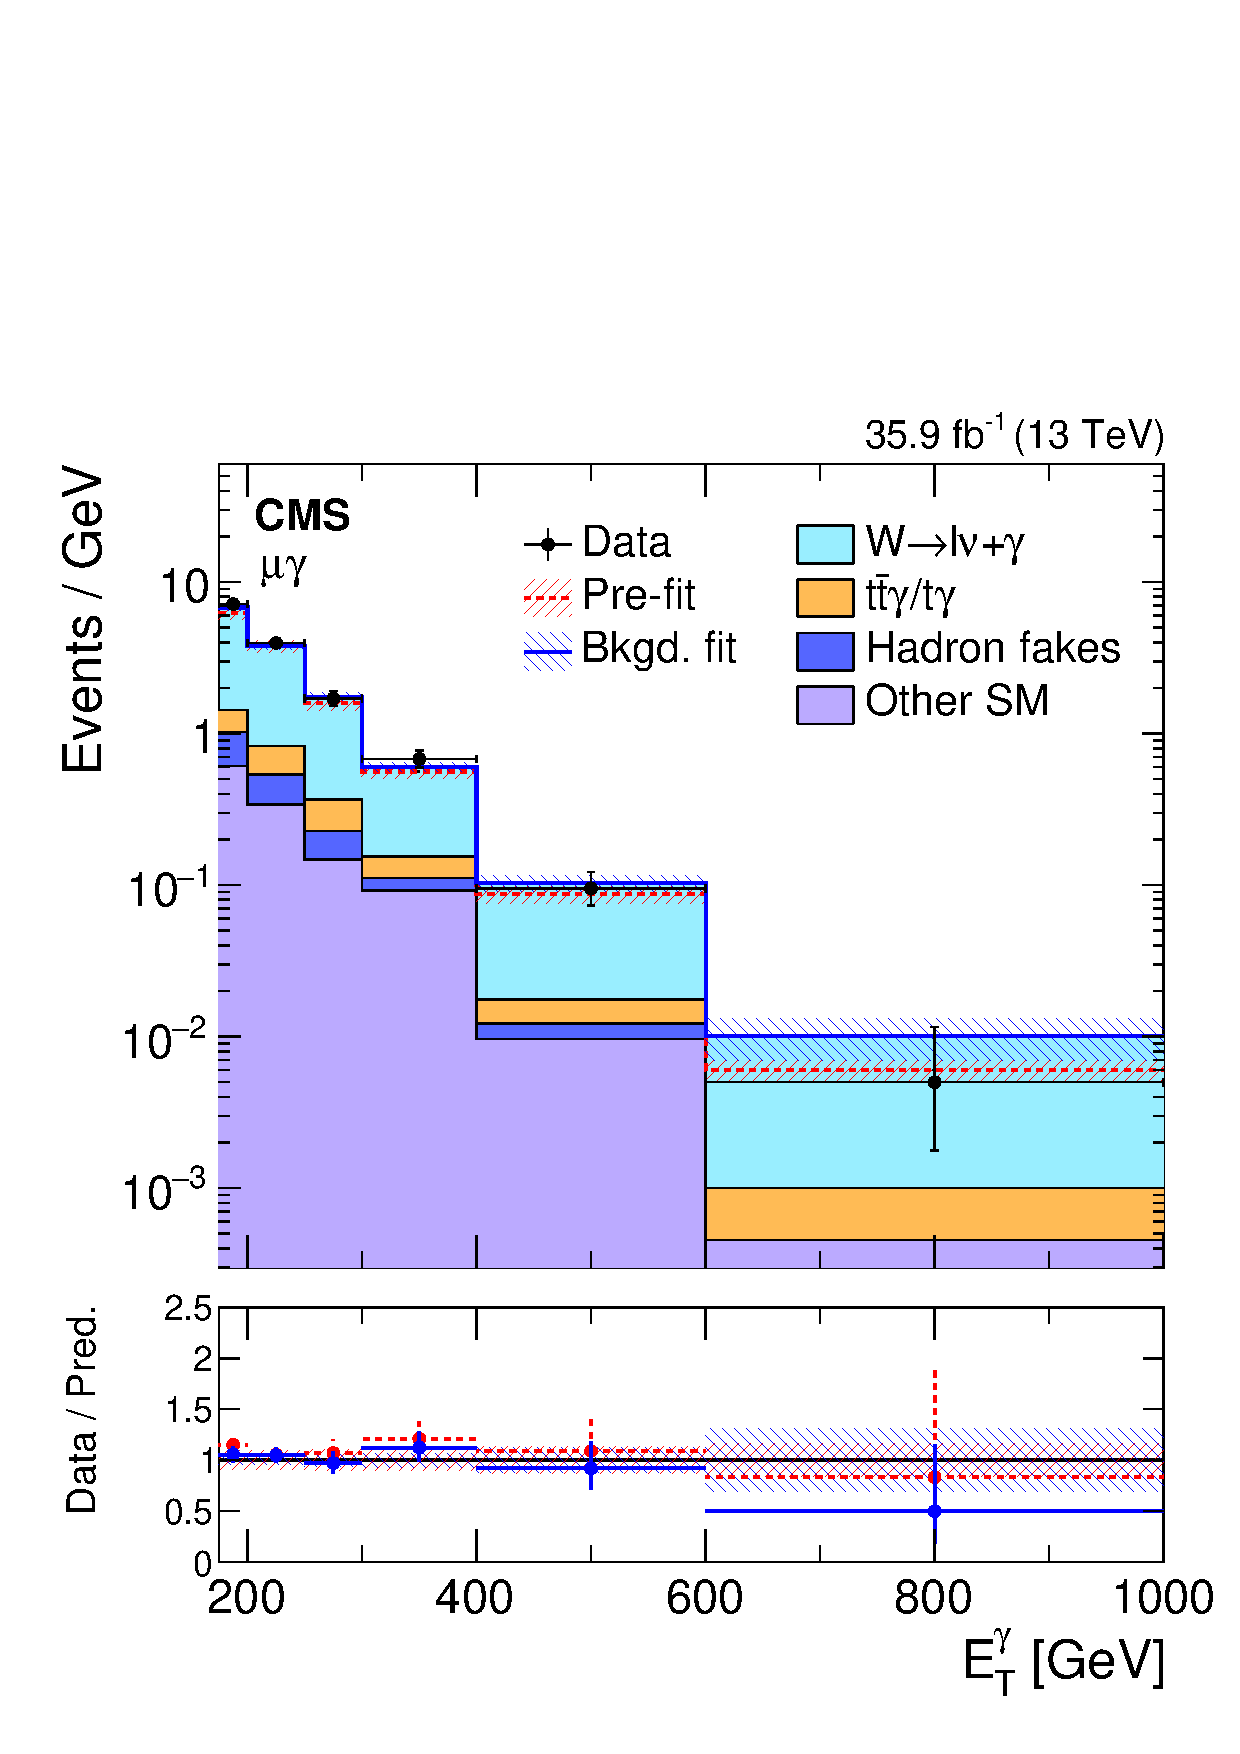
\includegraphics[width=0.45\textwidth]{figures/exo16053/Figure_005-d.pdf}
    \caption{
      Control region postfit \ETgamma\ distribution corresponding to the DM and ADD likelihood function:
      \Pe\Pe\Pgamma\ (top left), \Pmu\Pmu\Pgamma\ (top right), \Pe\Pgamma\ (bottom left), and
      \Pmu\Pgamma\ (bottom right). The last bin includes all events with $\ETgamma > 1000\unit{GeV}$.
      Published in~\cite{ref:JHEP02(2019)074}.
    }
    \label{fig:postfitDM_CR}
  \end{center}
\end{figure}

\begin{figure}[htbp]
  \begin{center}
    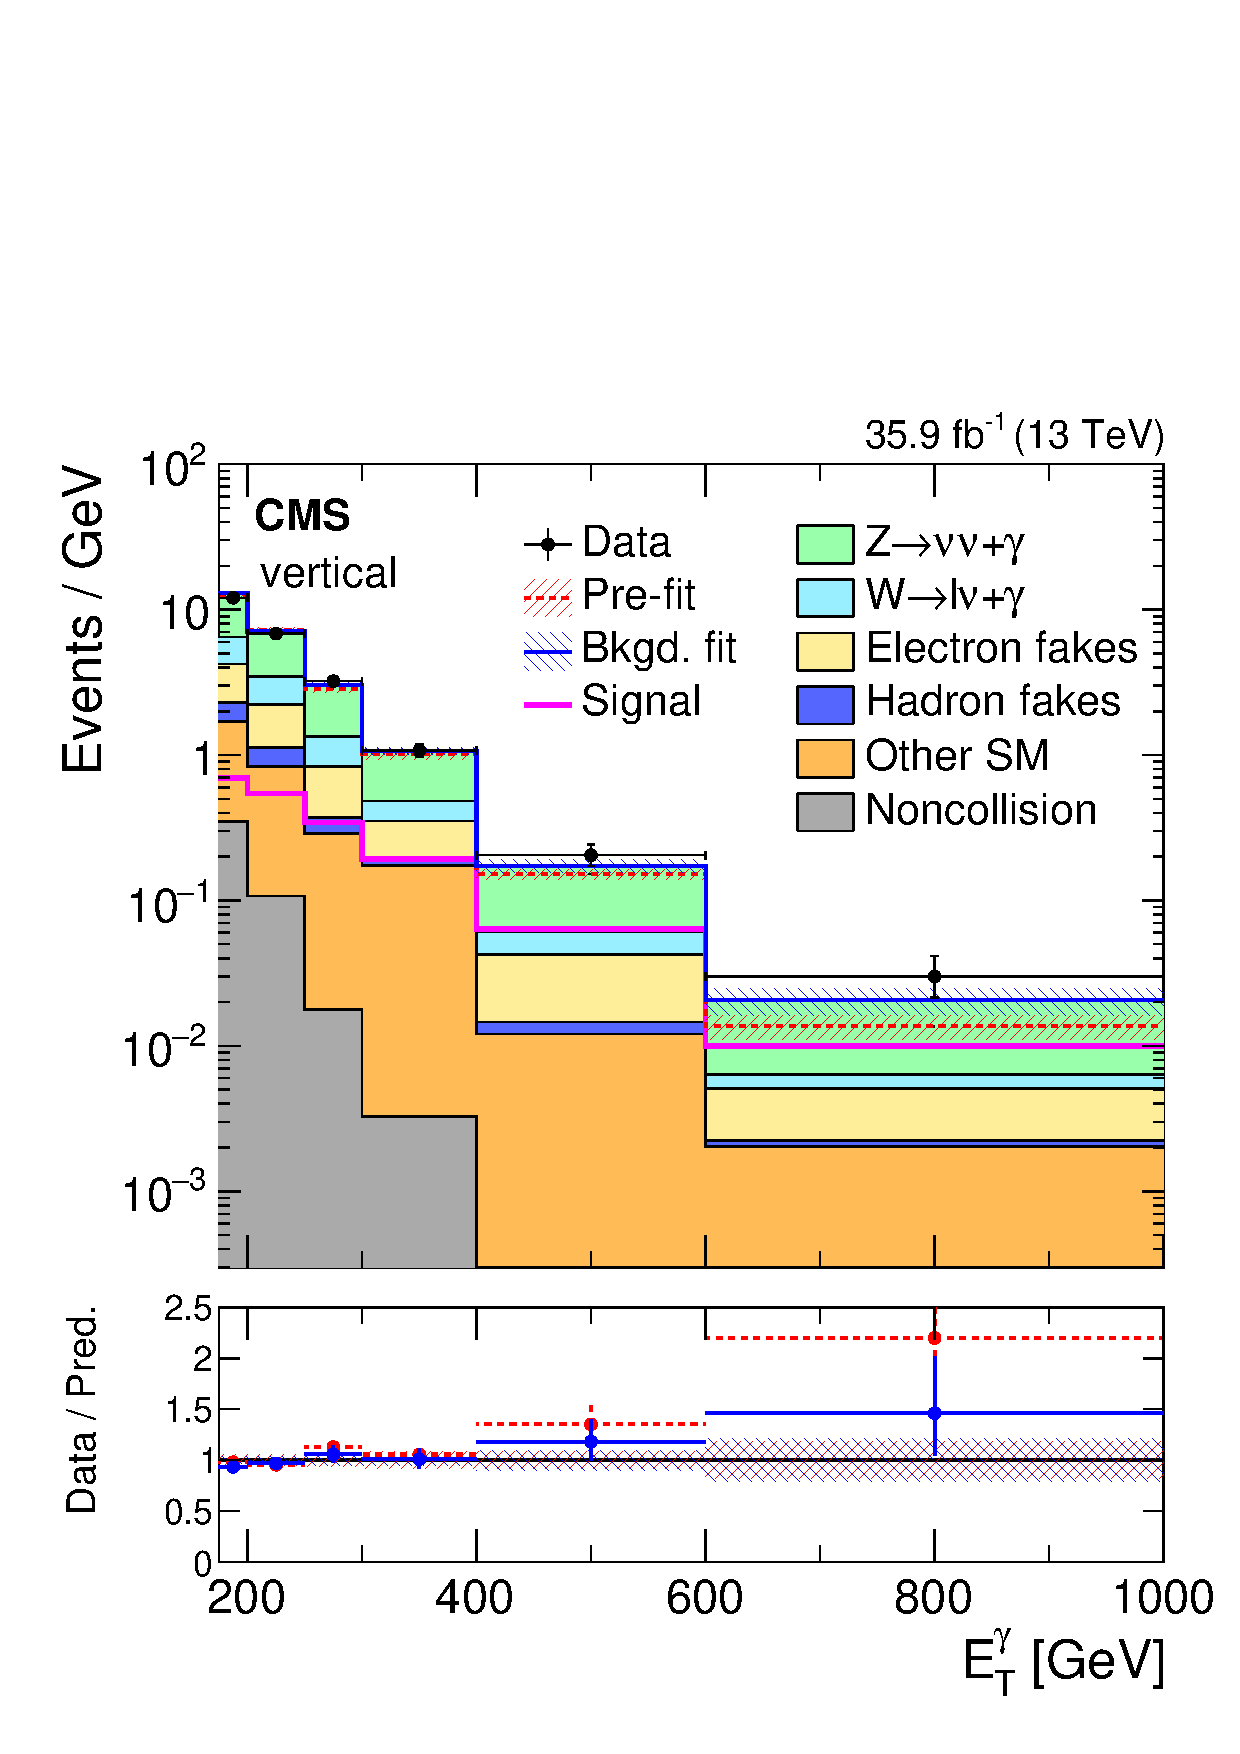
\includegraphics[width=0.45\textwidth]{figures/exo16053/Figure_006-b.pdf}
    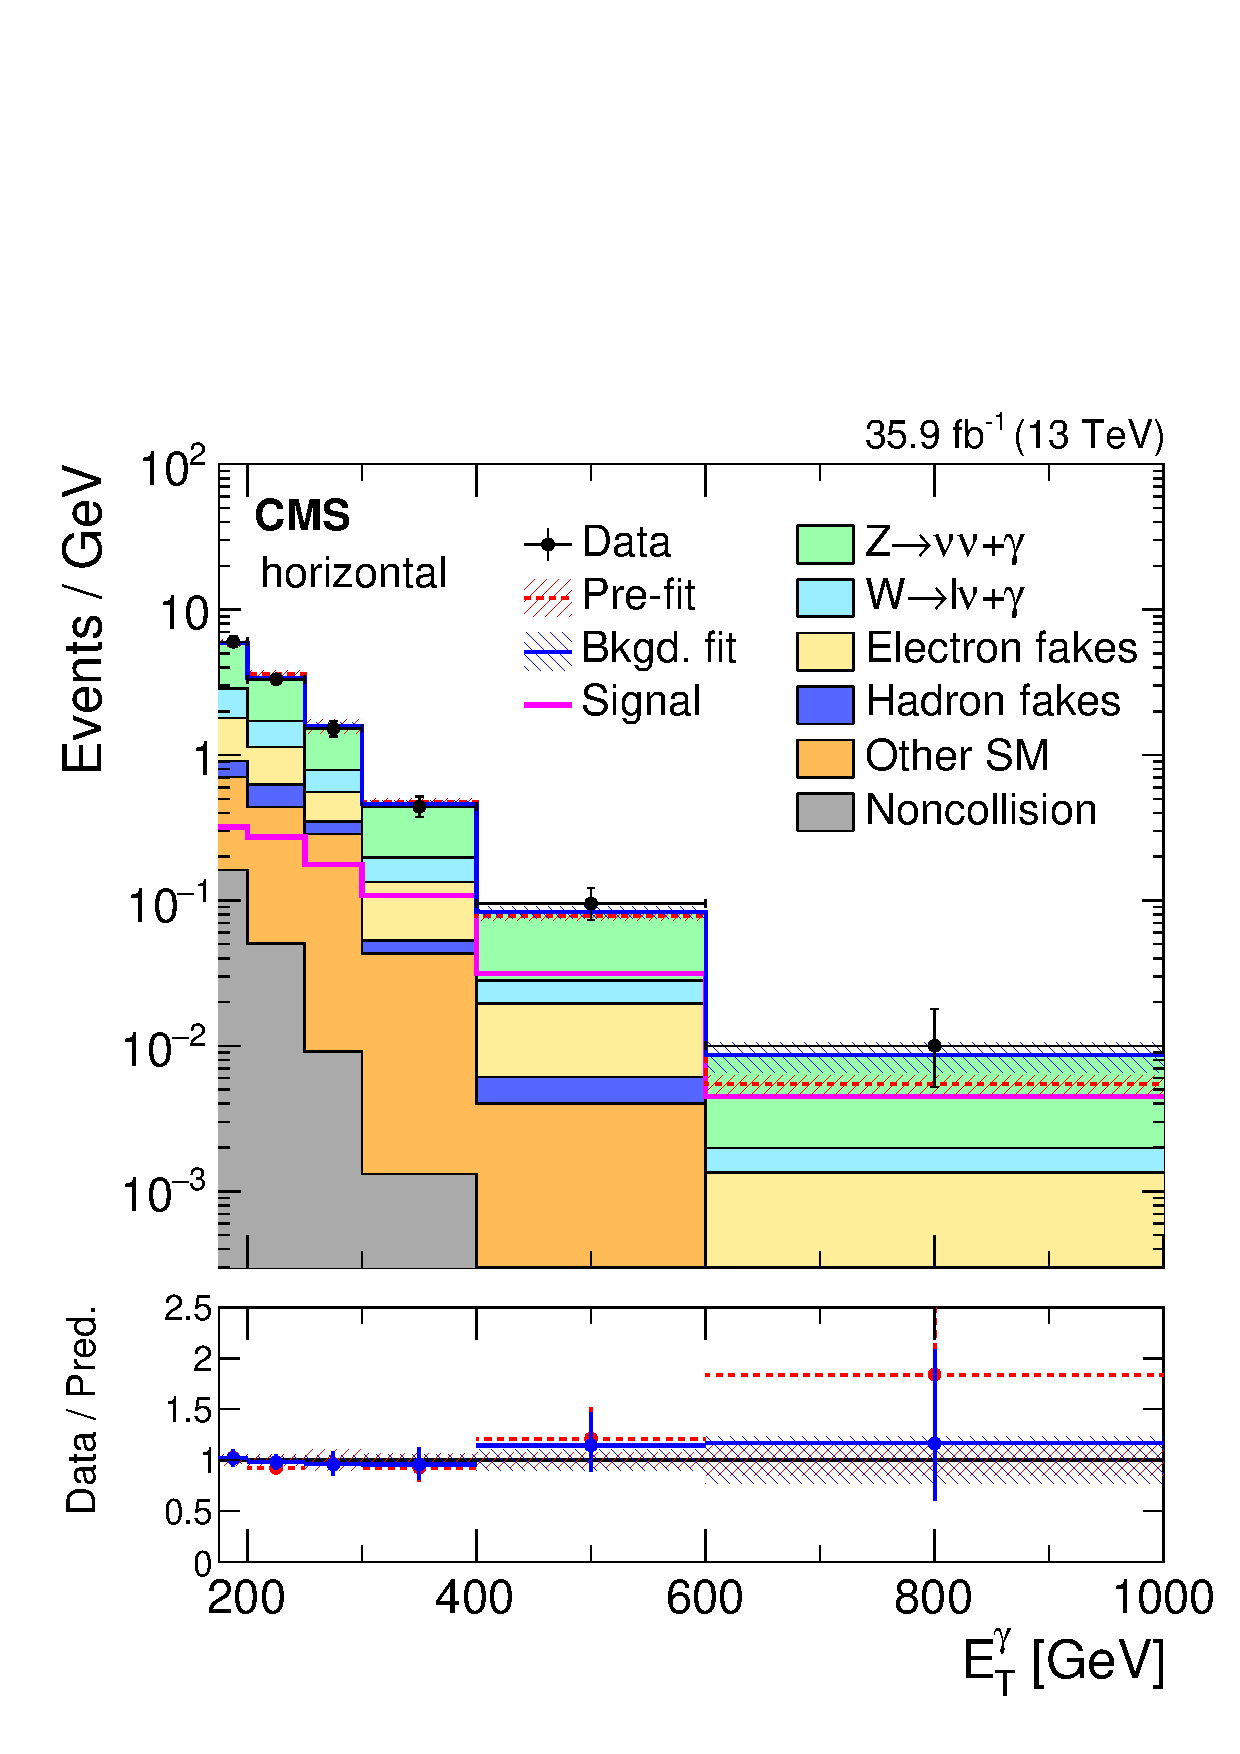
\includegraphics[width=0.45\textwidth]{figures/exo16053/Figure_006-a.pdf}
    \caption{
      Signal region postfit \ETgamma\ distributions corresponding to the DM and ADD likelihood function, with
      BSM signal strength set to zero: vertical region (left) and horizontal region (right). The last bin includes all events with $\ETgamma > 1000\unit{GeV}$.
      Published in~\cite{ref:JHEP02(2019)074}.
    }
    \label{fig:postfitDM_SR}
  \end{center}
\end{figure}

% \begin{figure}[htbp]
%   \begin{center}
%     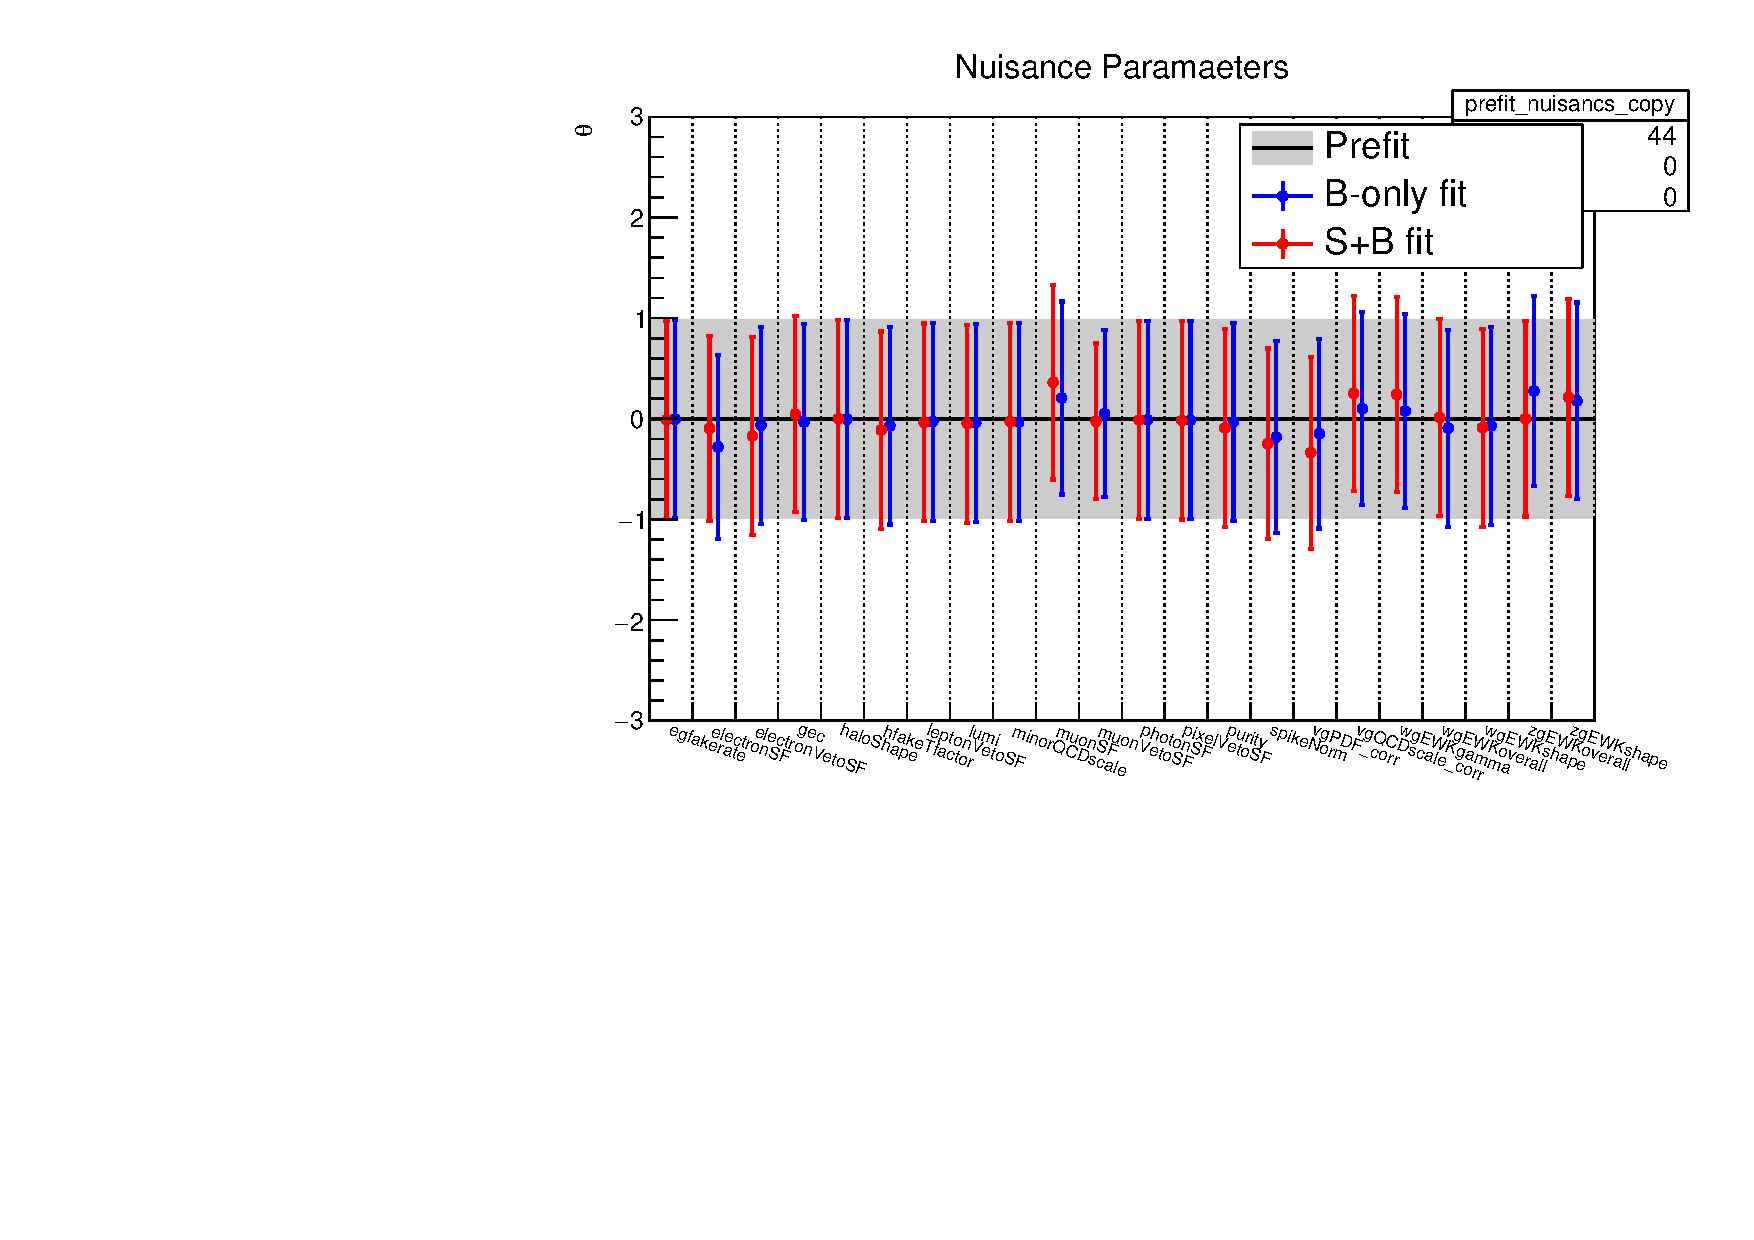
\includegraphics[width=0.675\textwidth]{figures/results/pulls_data_syst.pdf}
%     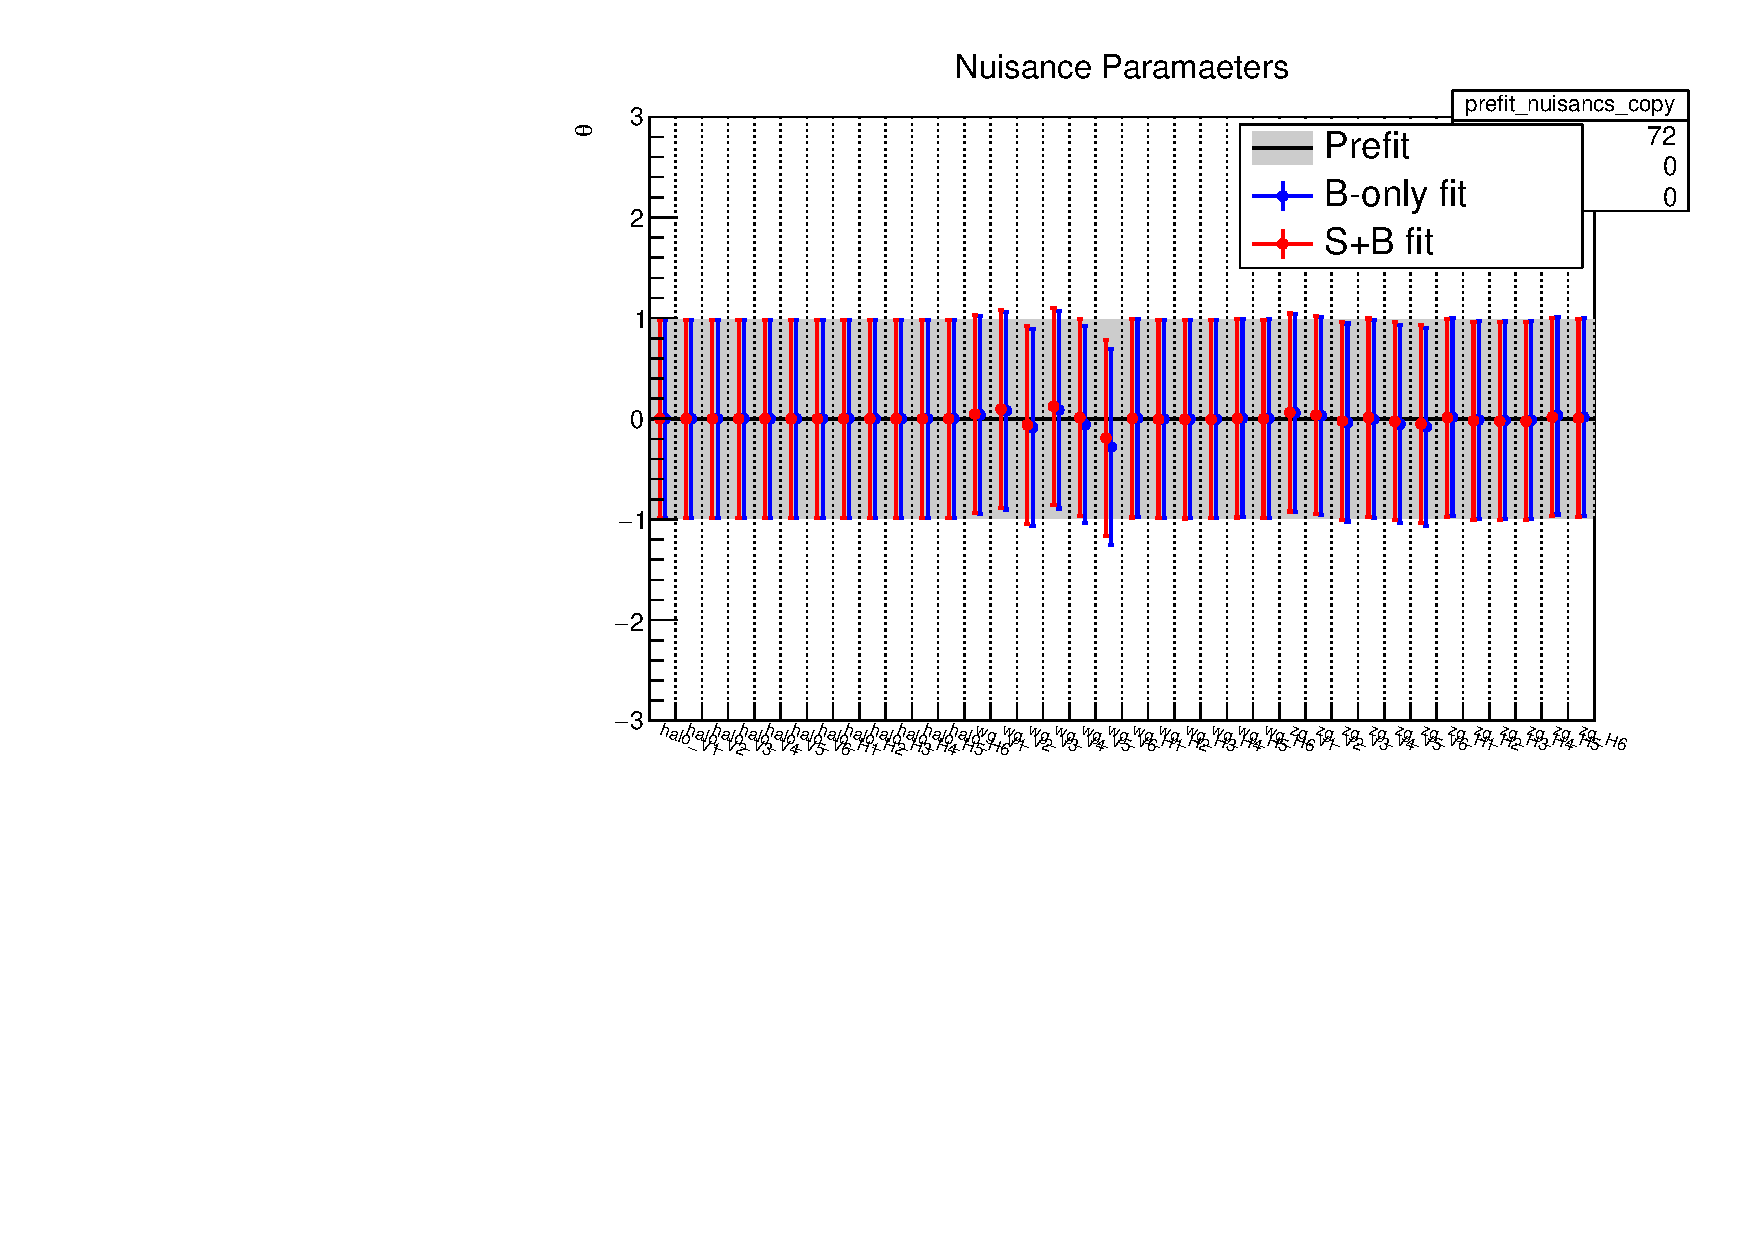
\includegraphics[width=0.675\textwidth]{figures/results/pulls_data_SR.pdf}
%     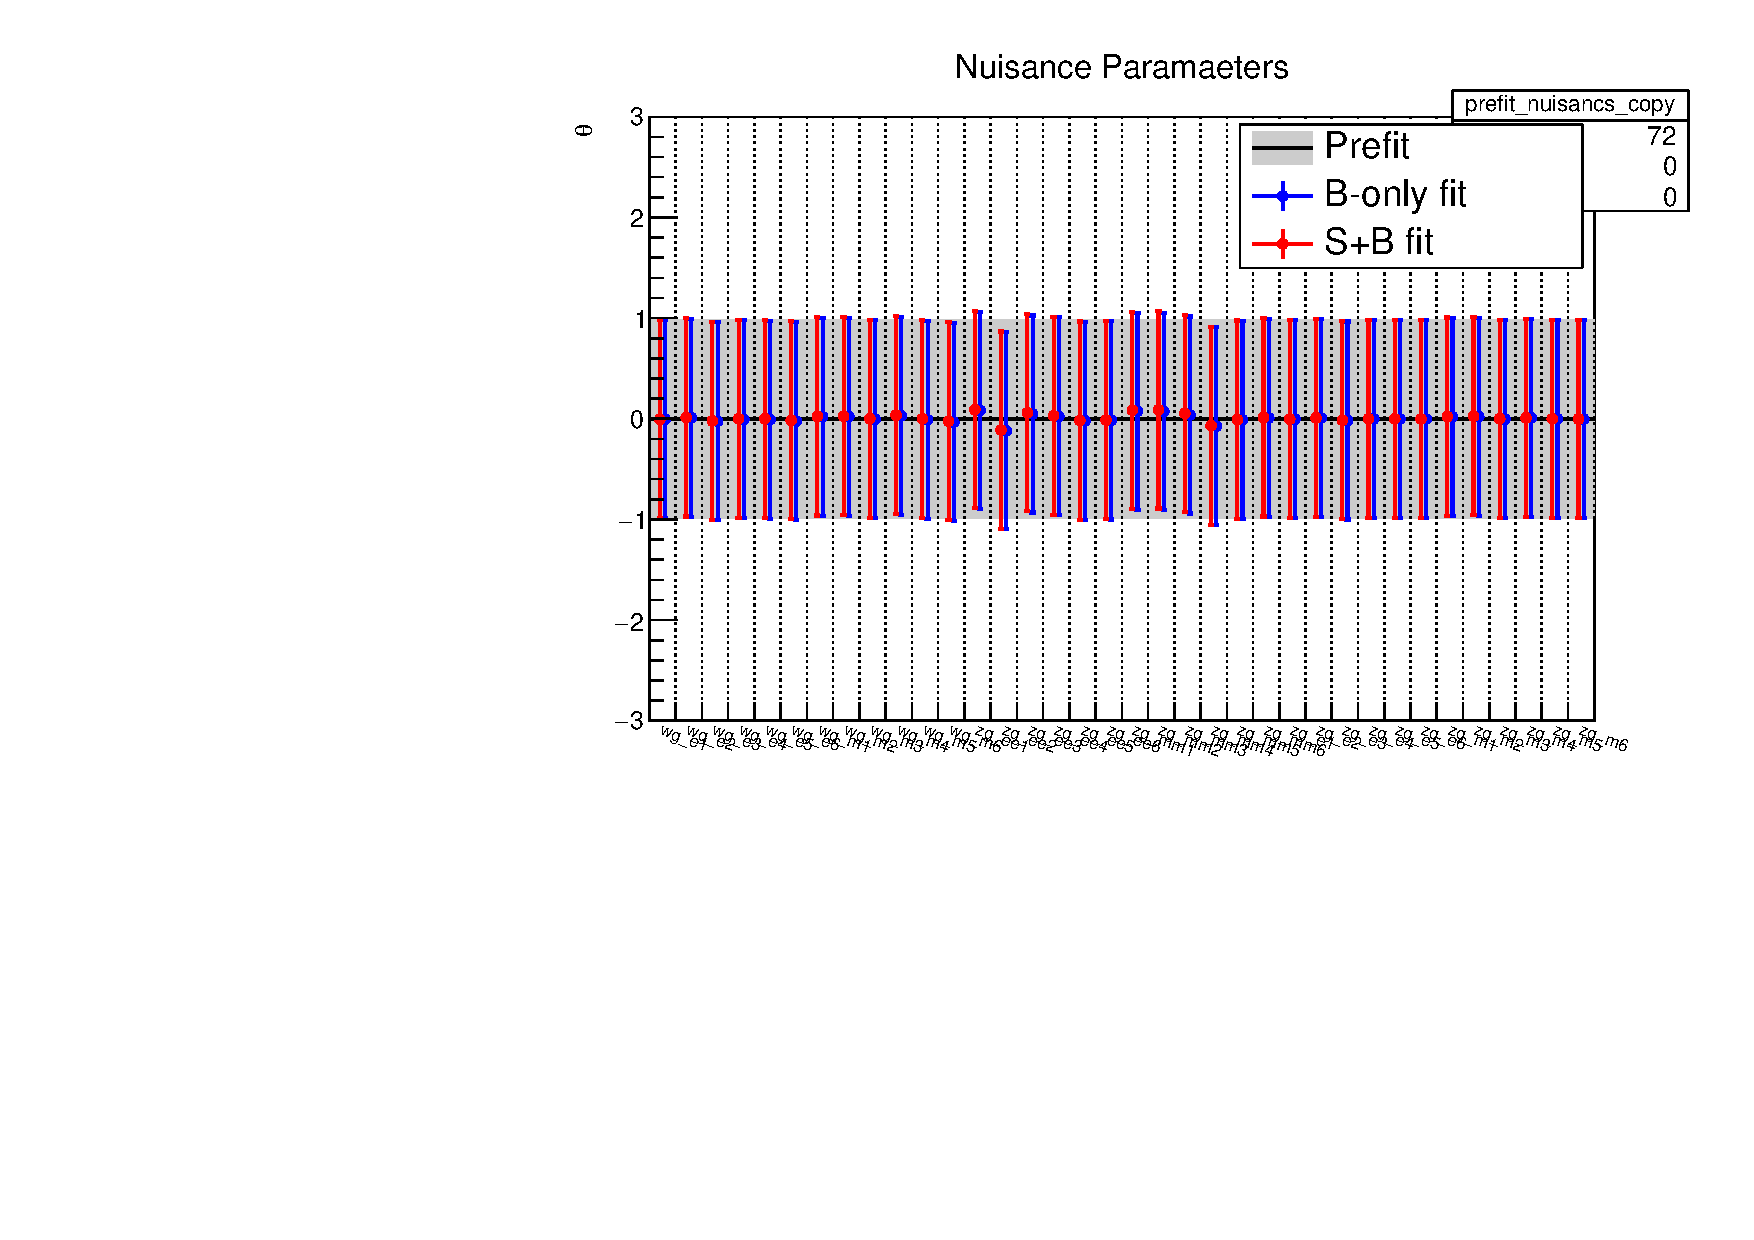
\includegraphics[width=0.675\textwidth]{figures/results/pulls_data_CR.pdf}
%     \caption{
%       Postfit nuisance pulls corresponding to the DM and ADD likelihood function.
%       Top: systematic uncertainties.
%       Middle: MC statistical uncertainties for the signal regions.
%       Bottom: MC statistical uncertainties for the control regions.
%     }
%     \label{fig:pullsDM}
%   \end{center}
% \end{figure}

% \begin{figure}[htbp]
%   \begin{center}
%     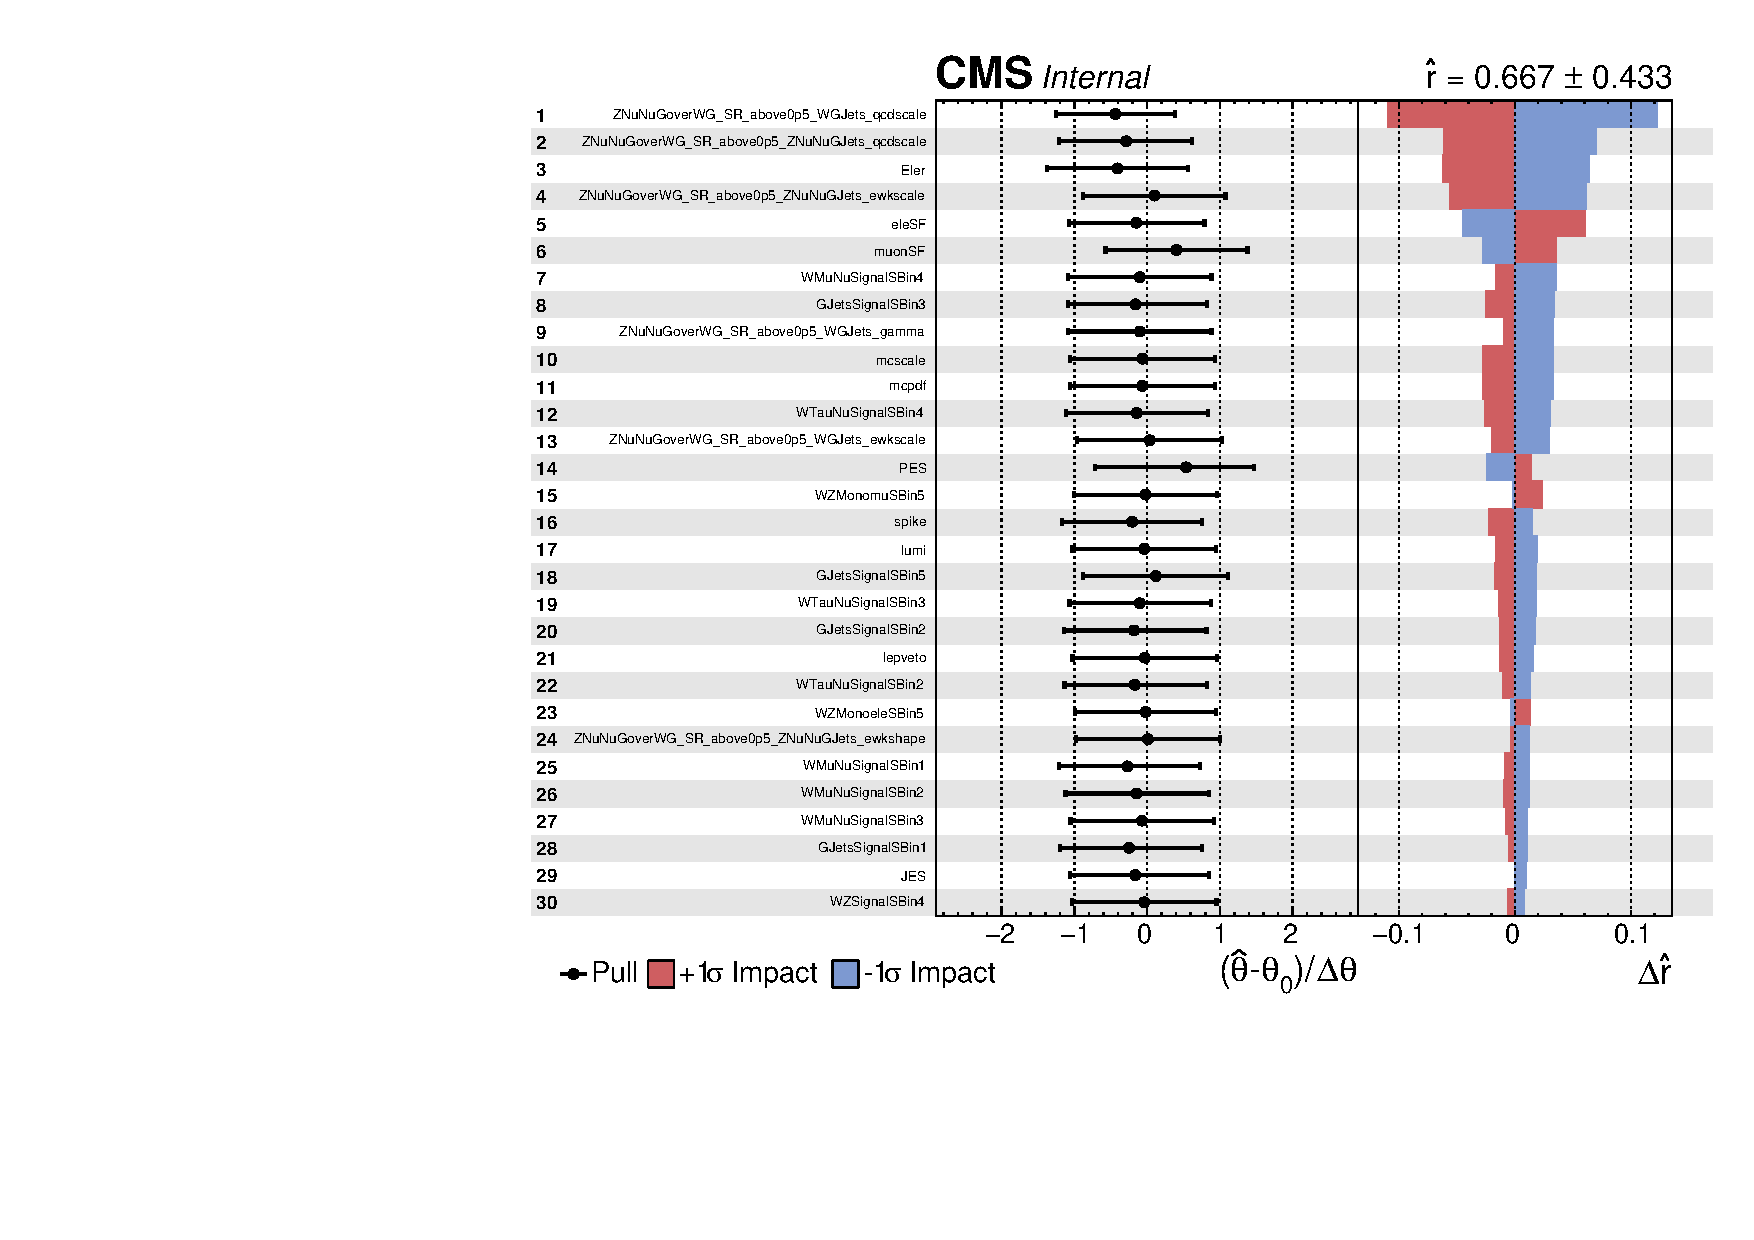
\includegraphics[width=0.85\textwidth]{figures/results/impacts_1.pdf}
%     \caption{
%       Impacts of the 30 leading nuisances on the 95\% CL upper limit of the signal strength $r$,
%       evaulated for the dark matter simplified model with vector mediator of mass 1000\unit{GeV}
%       and dark matter mass 1\unit{GeV}.
%     }
%     \label{fig:impacts1}
%   \end{center}
% \end{figure}

% Simulated DM simplified model samples with full CMS event reconstruction were generated at a few dozen mass points in the \Mmed--\Mdm\ mass plane. Redundant
% samples were generated to both LO and NLO in QCD.
% In order to more finely interpolate the exclusion limits on the DM simplified model parameters, additional DM samples were generated at
% 1800 mass points (900 each for Vector and Axial vector). These were each generated to LO in QCD, and without any
% subsequent detector simulation or event reconstruction. The overall cross section and the
% fraction of events falling in various bins of generated \pTgamma\ are estimated for each sample.
% A reweighting factor for the genPhoET distribution is then derived by taking the cross section times event fraction and dividing by
% the corresponding values for the nearest fully-reconstructed LO DM sample.  Choosing a mass point with a fully-reconstructed LO sample (the ``reference'' point)
% and applying the generated \pTgamma\ reweighting factor for another ``target'' point thereby gives an estimate of the \pTgamma\ distribution at the target
% point. These scale factors all appear to be linear, and they are each fit to a straight line to minimize the impact of statistical fluctuations.

% A second reweighting factor is obtained by taking the ratio of expected event yields for fully-simulated NLO and LO DM samples as a function of
% reconstructed \ETgamma, for events passing the full signal region selection criteria. This \ETgamma-binned ratio is also fit to a straight line.
% Applying this reweighting factor to the reconstructed \ETgamma\ distribution from the LO sample gives an estimate of what this distribution
% would look like for a sample generated to NLO. Thus, applying both the genPhoPT and recoPhoET reweighting factors to a fully reconstructed
% LO sample at some reference point gives an estimate of the recoPhoET distribution for an NLO sample at a target point.

\begin{figure}[htbp]
  \begin{center}
   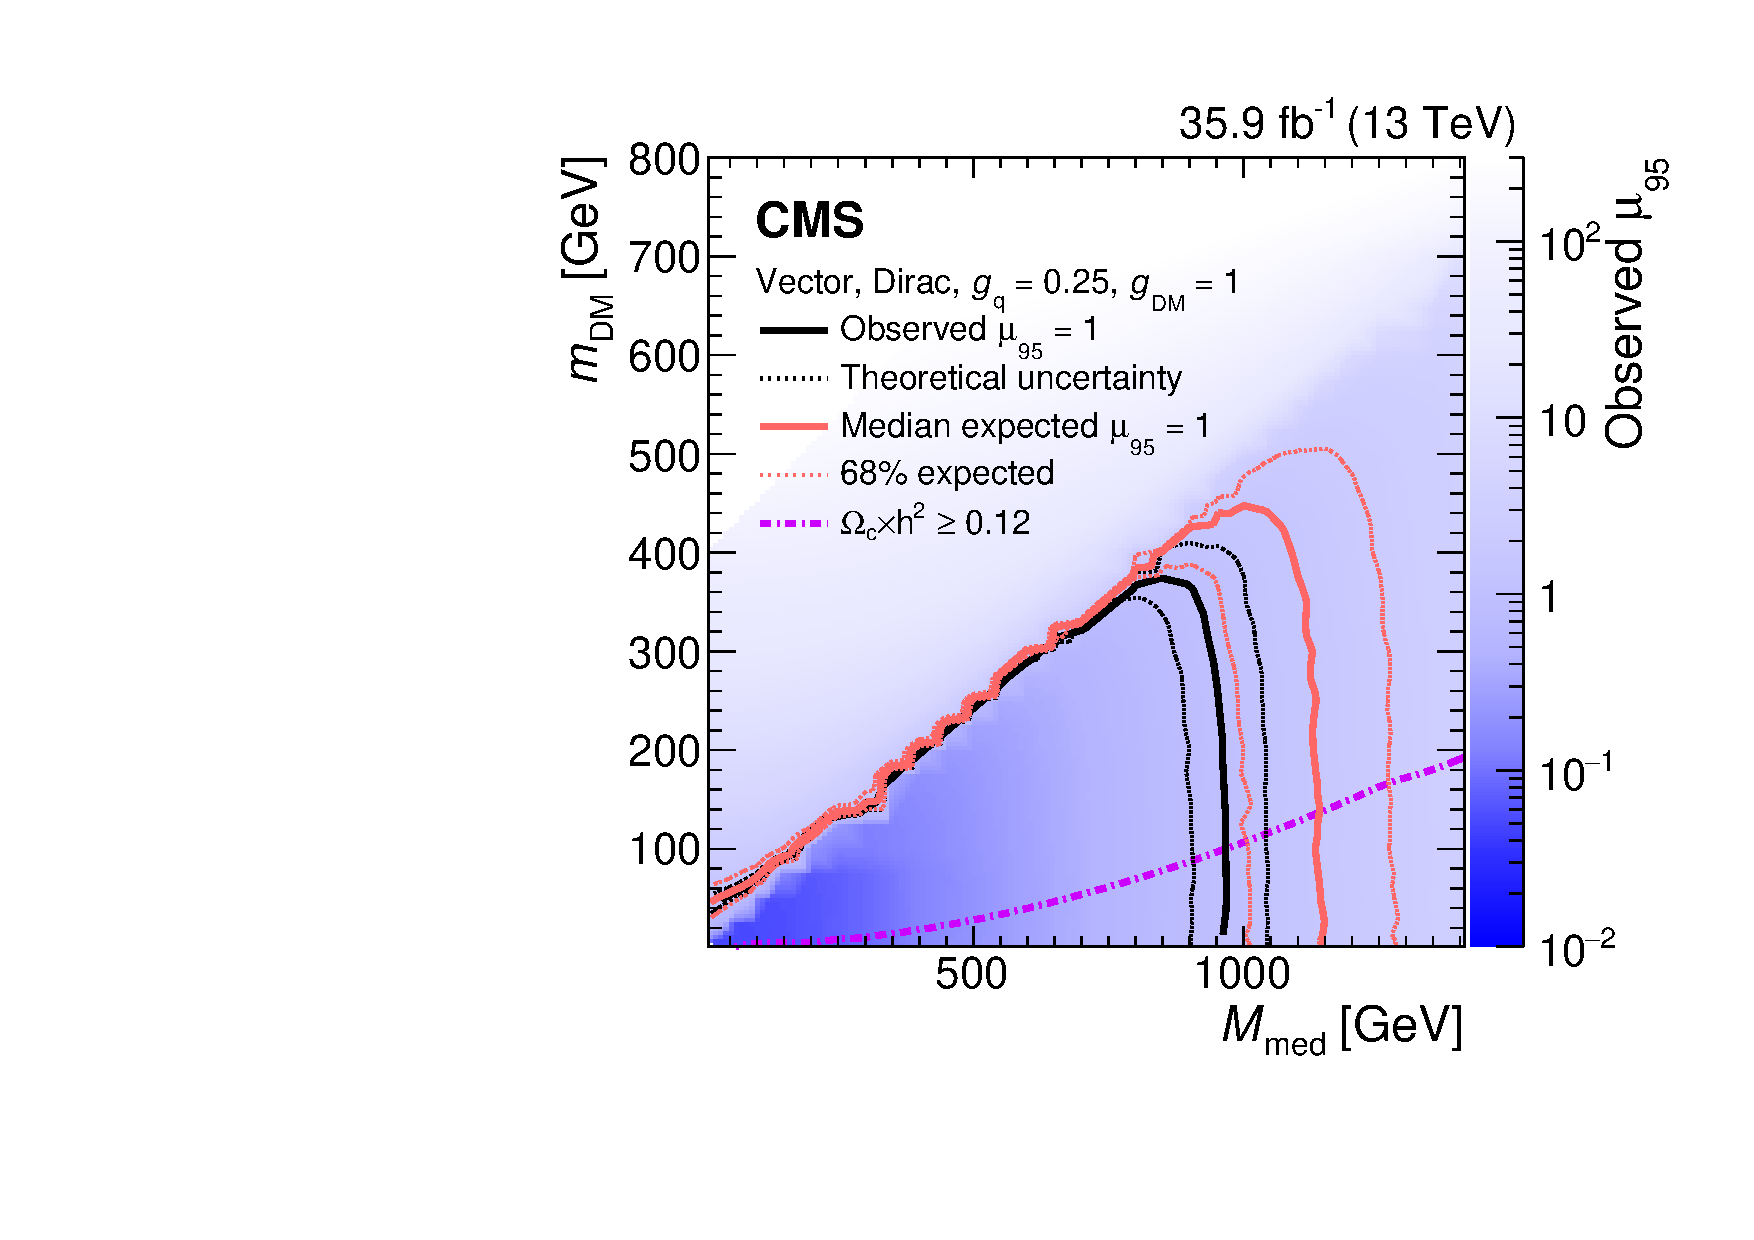
\includegraphics[width=0.48\linewidth]{figures/exo16053/Figure_007-a.pdf}
    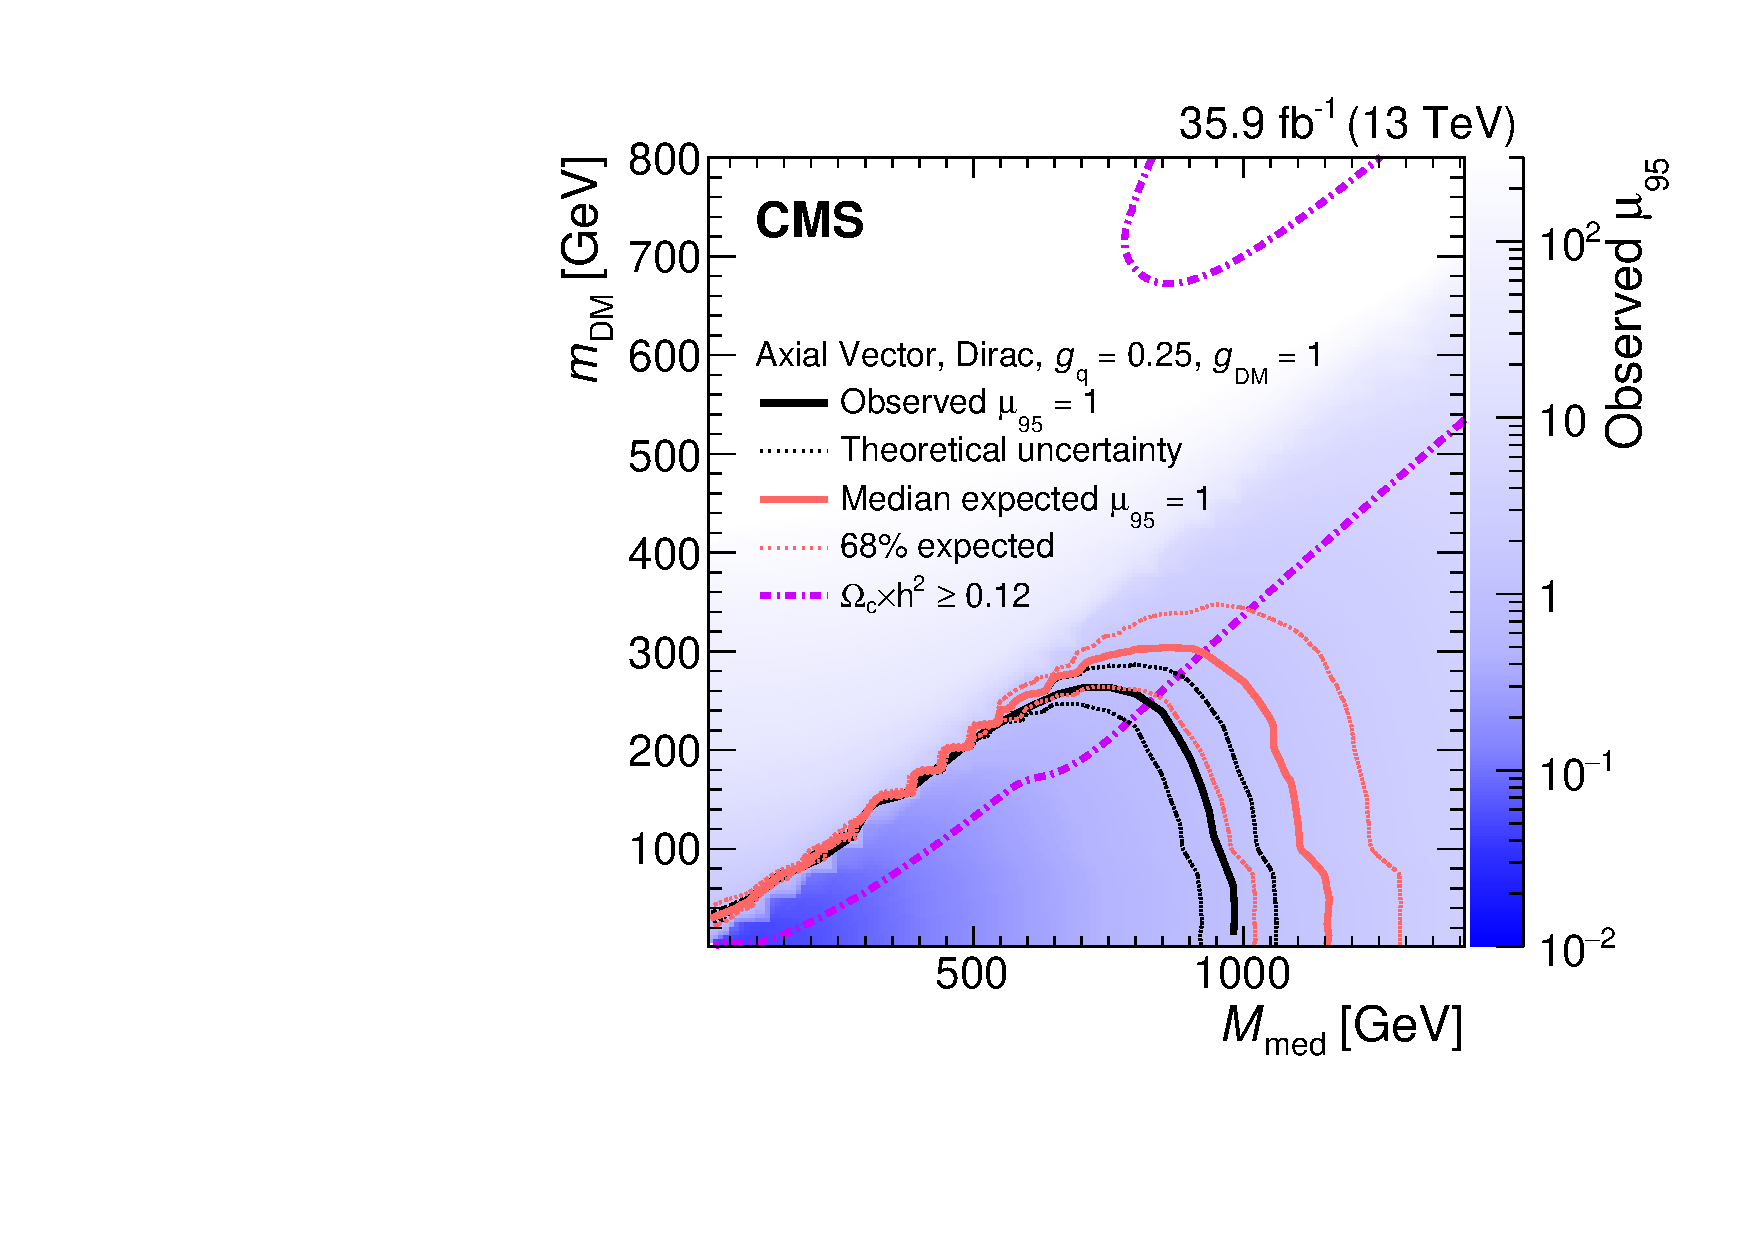
\includegraphics[width=0.48\linewidth]{figures/exo16053/Figure_007-b.pdf}
    \caption{
      The ratio of 95\% CL cross section upper limits to theoretical cross section ($\mu_{95}$), for DM simplified models with vector (left) and axial-vector
      (right) mediators, assuming $\gq=0.25$ and $\gdm=1$. Observed and expected $\mu_{95} = 1$ contours are overlaid.
      The region below the observed contour is excluded at 95\% CL or above. Published in~\cite{ref:JHEP02(2019)074}.
    }
    \label{fig:2d_mm}
  \end{center}
\end{figure}

Figure~\ref{fig:2d_mx} shows the exclusion contours translated into the
$\sigma_{\text{SI/SD}}$--\mdm\ plane, where $\sigma_{\text{SI/SD}}$ are the
spin-independent/dependent DM--nucleon scattering cross sections, respectively.
This translation and its graphical presentation follow the prescriptions given in Ref.~\cite{ref:1603.04156}.
In particular, to enable direct comparisons with results
from DD experiments, these limits are calculated at 90\% CL~\cite{ref:1507.00966}.
Relative to DD experiments, this search establishes stronger constraints for $\mdm < 2\unit{GeV}$ (spin-independent), 200\unit{GeV}
(spin-dependent), for the model parameters assumed here.

\begin{figure}[htbp]
  \begin{center}
    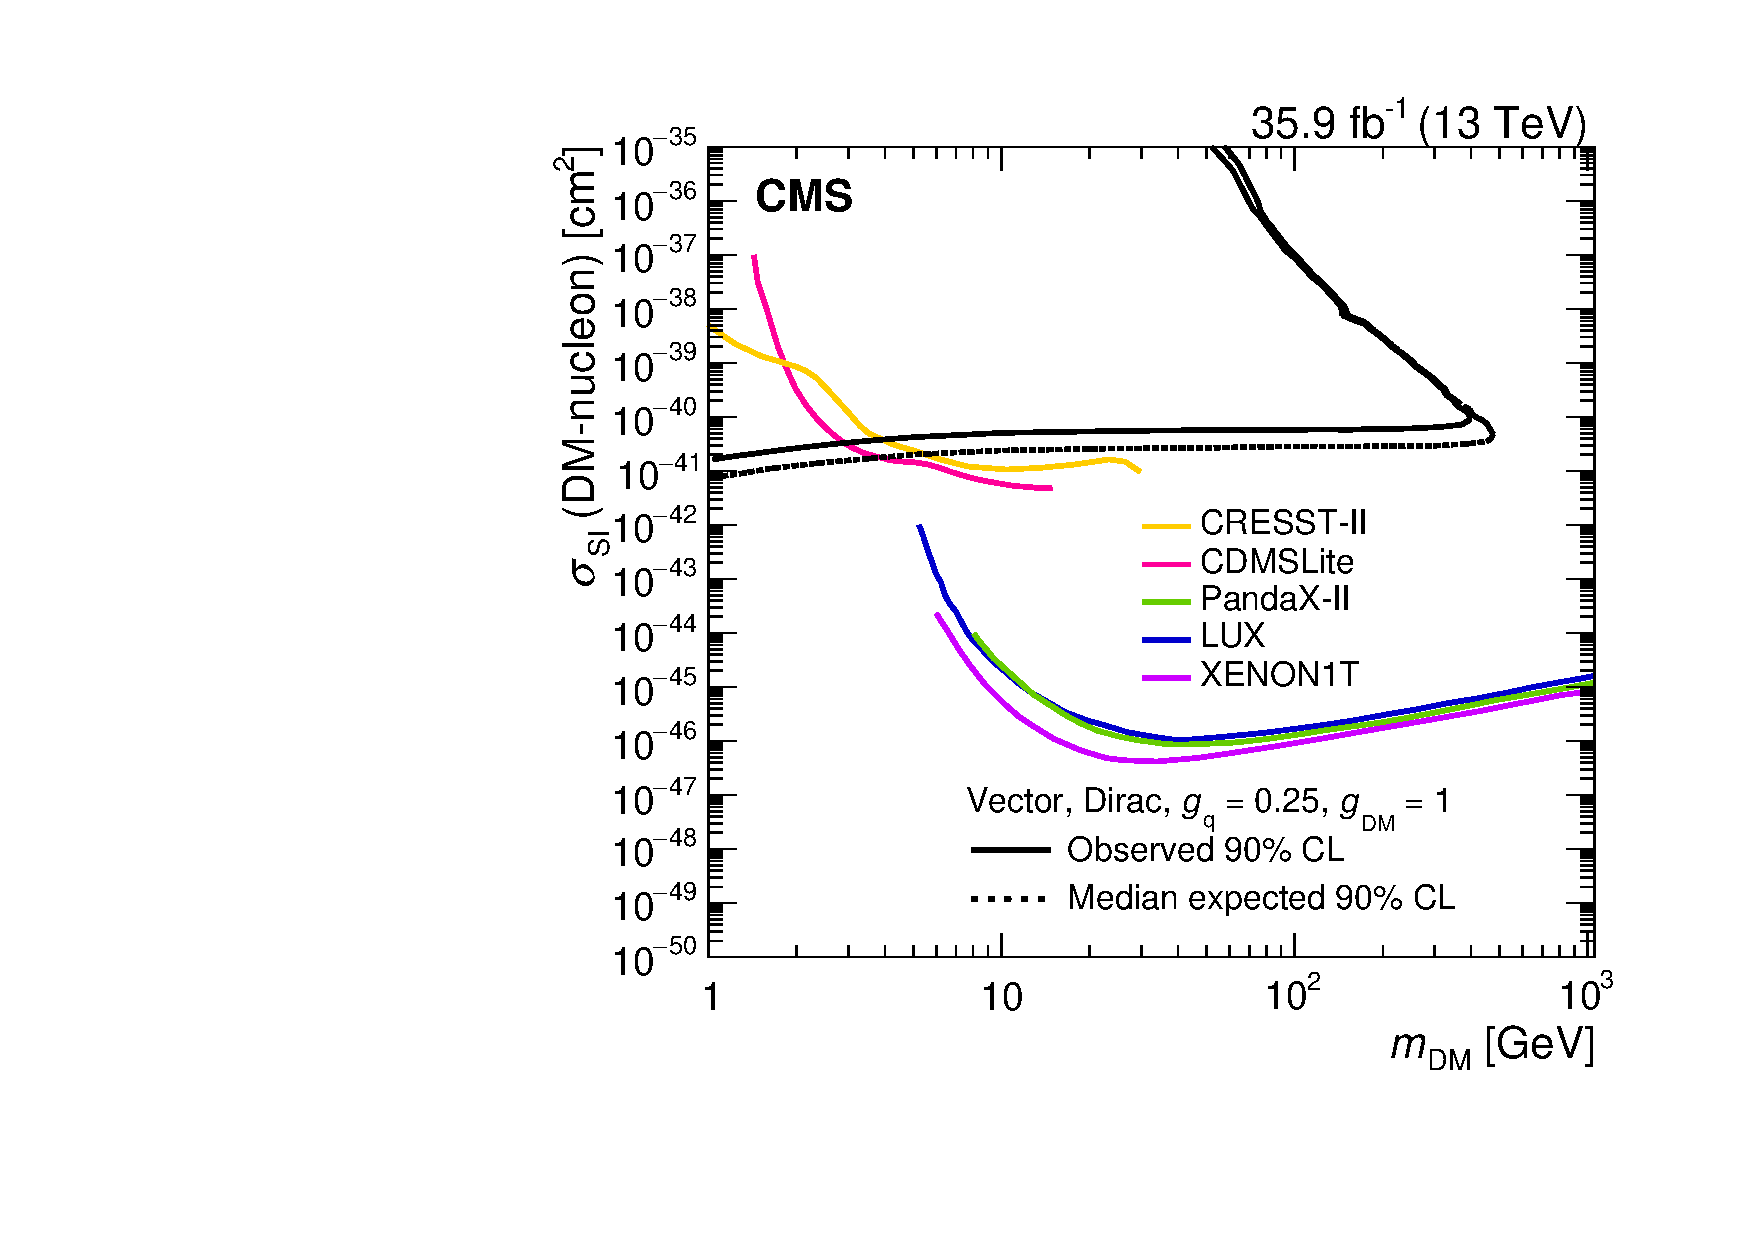
\includegraphics[width=0.48\linewidth]{figures/exo16053/Figure_008-a.pdf}
    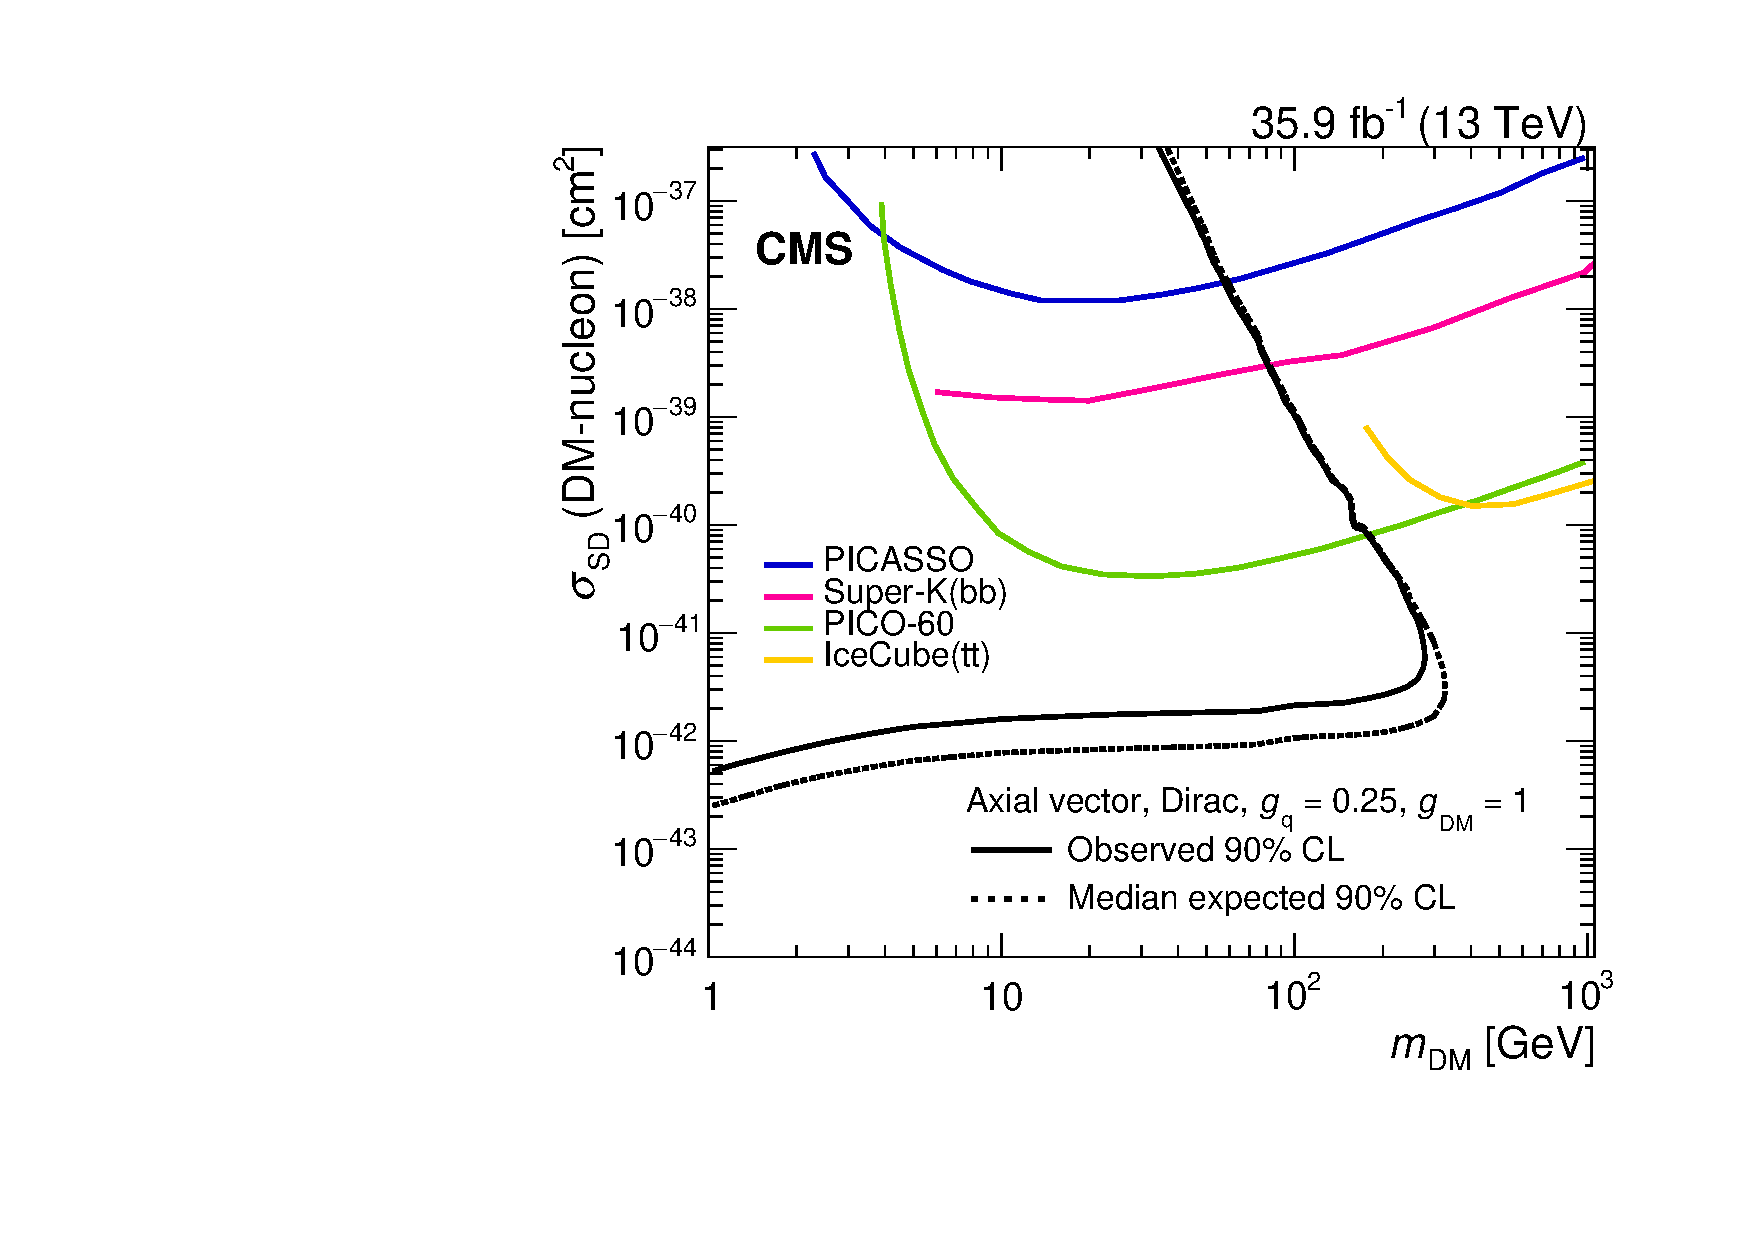
\includegraphics[width=0.48\linewidth]{figures/exo16053/Figure_008-b.pdf}
    \caption{
      The 90\% CL exclusion limits on the DM--nucleon spin-independent (left)
      and spin-dependent (right) scattering cross sections involving vector and axial-vector mediators, respectively,
      as a function of \mdm. Simplified model parameters of $\gq=0.25$ and $\gdm=1$ are assumed.
      The region to the upper left of the contour is excluded at 95\% CL or above. Published in~\cite{ref:JHEP02(2019)074}.
    }
    \label{fig:2d_mx}
  \end{center}
\end{figure}

Upper limits on the cross section for the DM--EWK EFT model are translated into the lower limits on the suppression scale $\Lambda$, shown in
Fig.~\ref{fig:DMEWKlimits}. The EFT hypothesis is excluded at $95\%$ CL or above for values of $\Lambda$ up to 850\unit{GeV} (observed), 950\unit{GeV}
(expected), at small \mdm\ values.

\begin{figure}[htbp]
\begin{center}
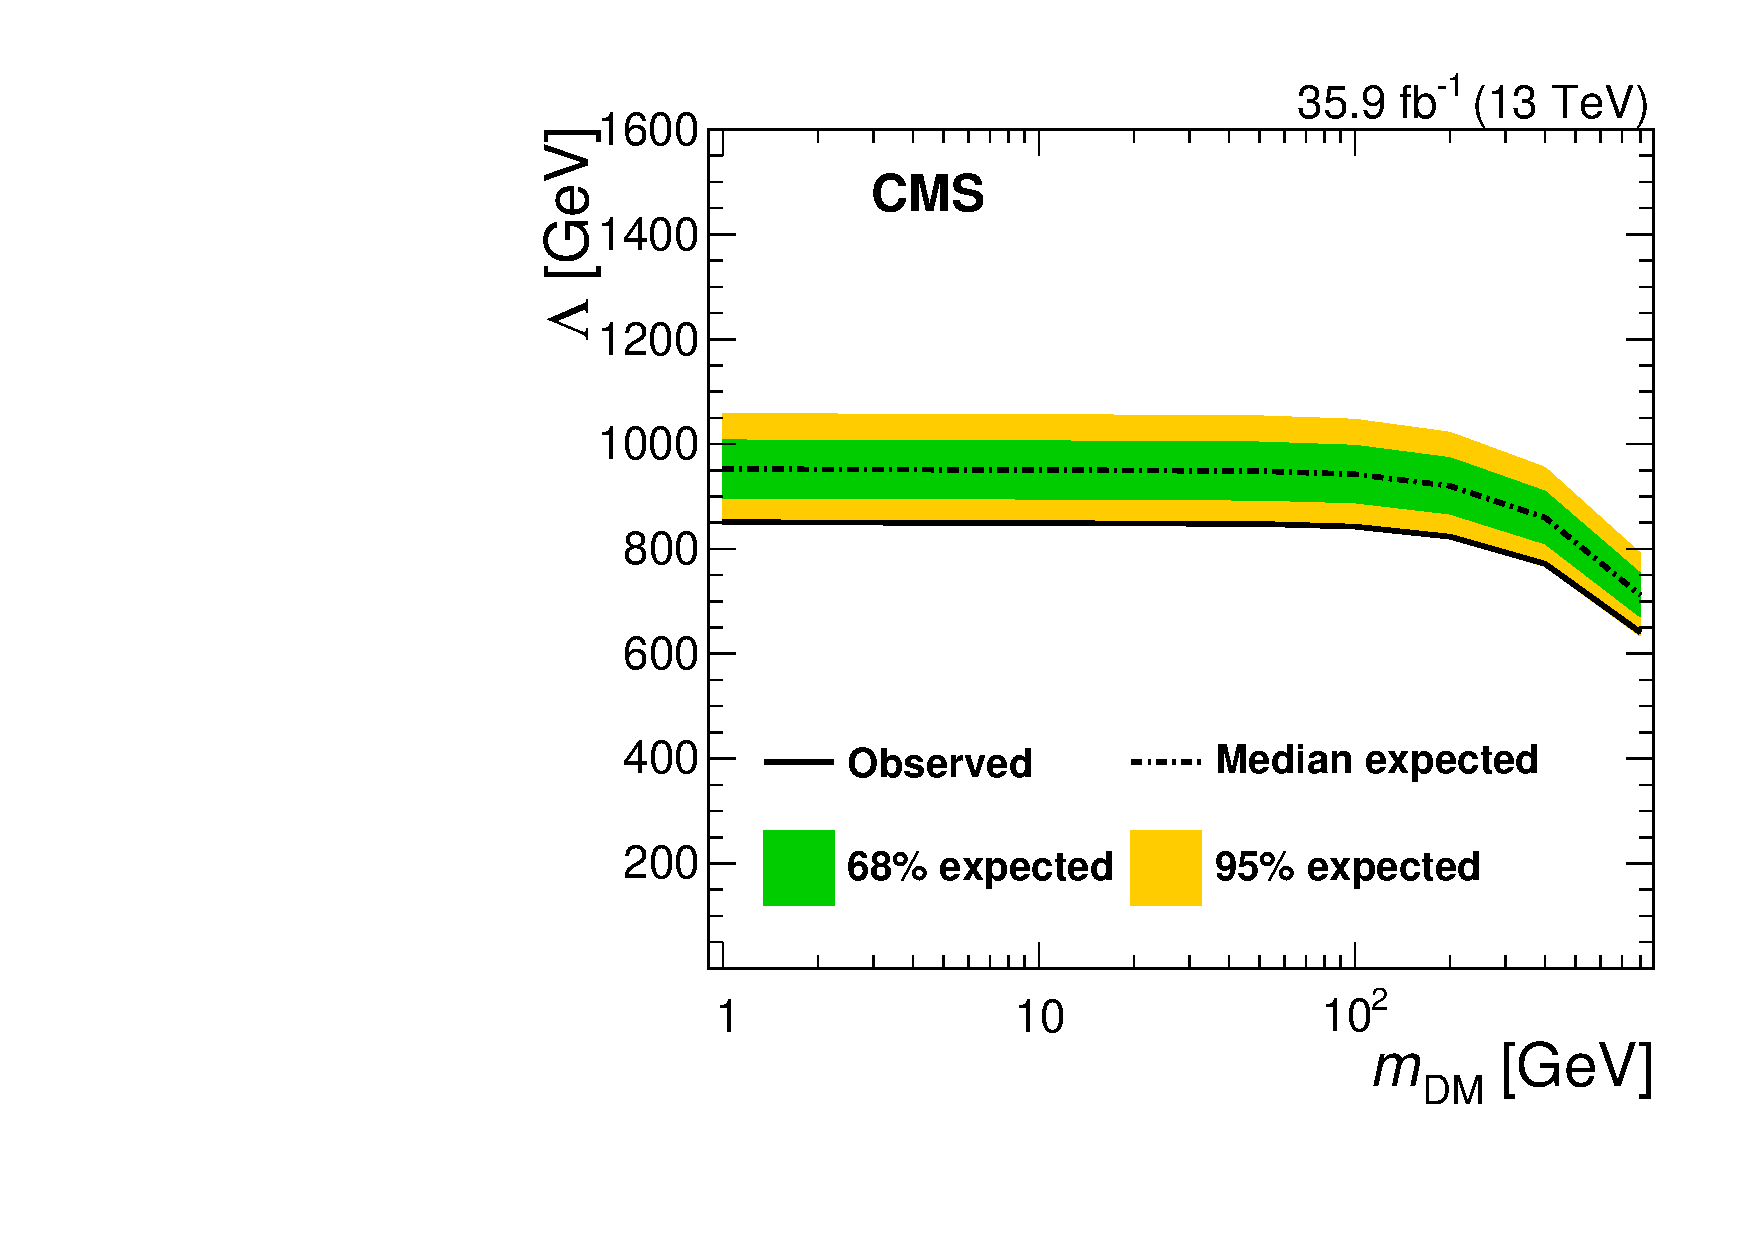
\includegraphics[width=7.5cm,height=7.0cm]{figures/exo16053/Figure_009.pdf}
\caption{The 95\% CL observed and expected lower limits on $\Lambda$ for the DM--EWK EFT model, shown as a function of \mdm.
Published in~\cite{ref:JHEP02(2019)074}.}
\label{fig:DMEWKlimits}
\end{center}
\end{figure}

\section{ADD limits} \label{sec:results_ADD}
The postfit plots for the ADD likelihood function (with BSM signal strength fixed to zero) are identical
to those shown in sec.~\ref{sec:results_DM}. Figure~\ref{fig:ADDLimits} shows the upper limit on the ADD cross section as well as its
theoretically calculated value for $n=3$ extra dimensions, as a function of \mD. The ADD hypothesis is excluded at 95\% CL or above in the region
where the theoretical curve is higher than the observed upper limit, corresponding to values of \mD\ up to 2.85\unit{TeV}.
Lower limits on \mD\ for various different values of $n$ are listed in Table~\ref{tab:MDLimits}, and graphically illustrated in Fig.~\ref{fig:MDLimits}.

\begin{figure}[htbp]
  \begin{center}
    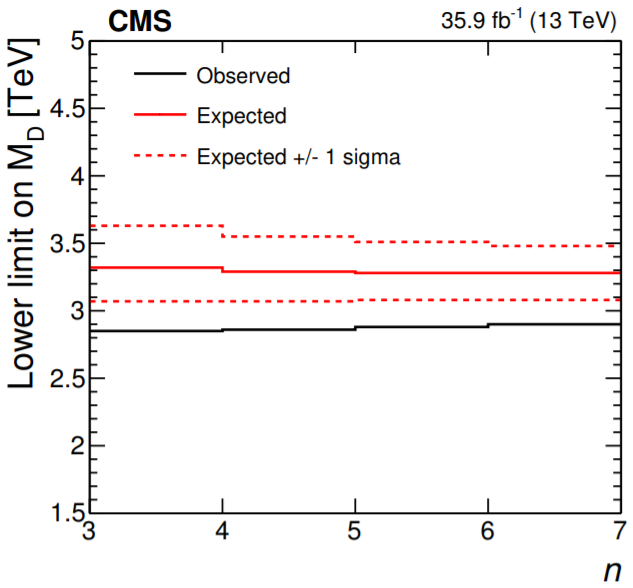
\includegraphics[width=0.5\textwidth]{figures/exo16053/add.png}
    \caption{The 95\% CL upper limits on the ADD graviton production cross section, as a function of \mD\, for $n=3$ extra dimensions.
    Published in~\cite{ref:JHEP02(2019)074}.}
    \label{fig:ADDLimits}
  \end{center}
\end{figure}

\begin{table}[htbp]
  \begin{center}
    \label{tab:MDLimits}
    \begin{tabular}{|c|c|c|}
      \hline
      $n$ & Obs. limit [TeV] & Exp. limit [TeV] \\
      \hline
      3 & 2.85 & 3.32 \\
      4 & 2.86 & 3.29 \\
      5 & 2.88 & 3.28\\
      6 & 2.90 & 3.28 \\
      \hline
    \end{tabular}
    \caption{The 95\% CL observed and expected lower limits on the ADD mass scale \mD\ as a function of $n$, the number of extra dimensions.}
  \end{center}
\end{table}

\begin{figure}[htbp]
  \begin{center}
    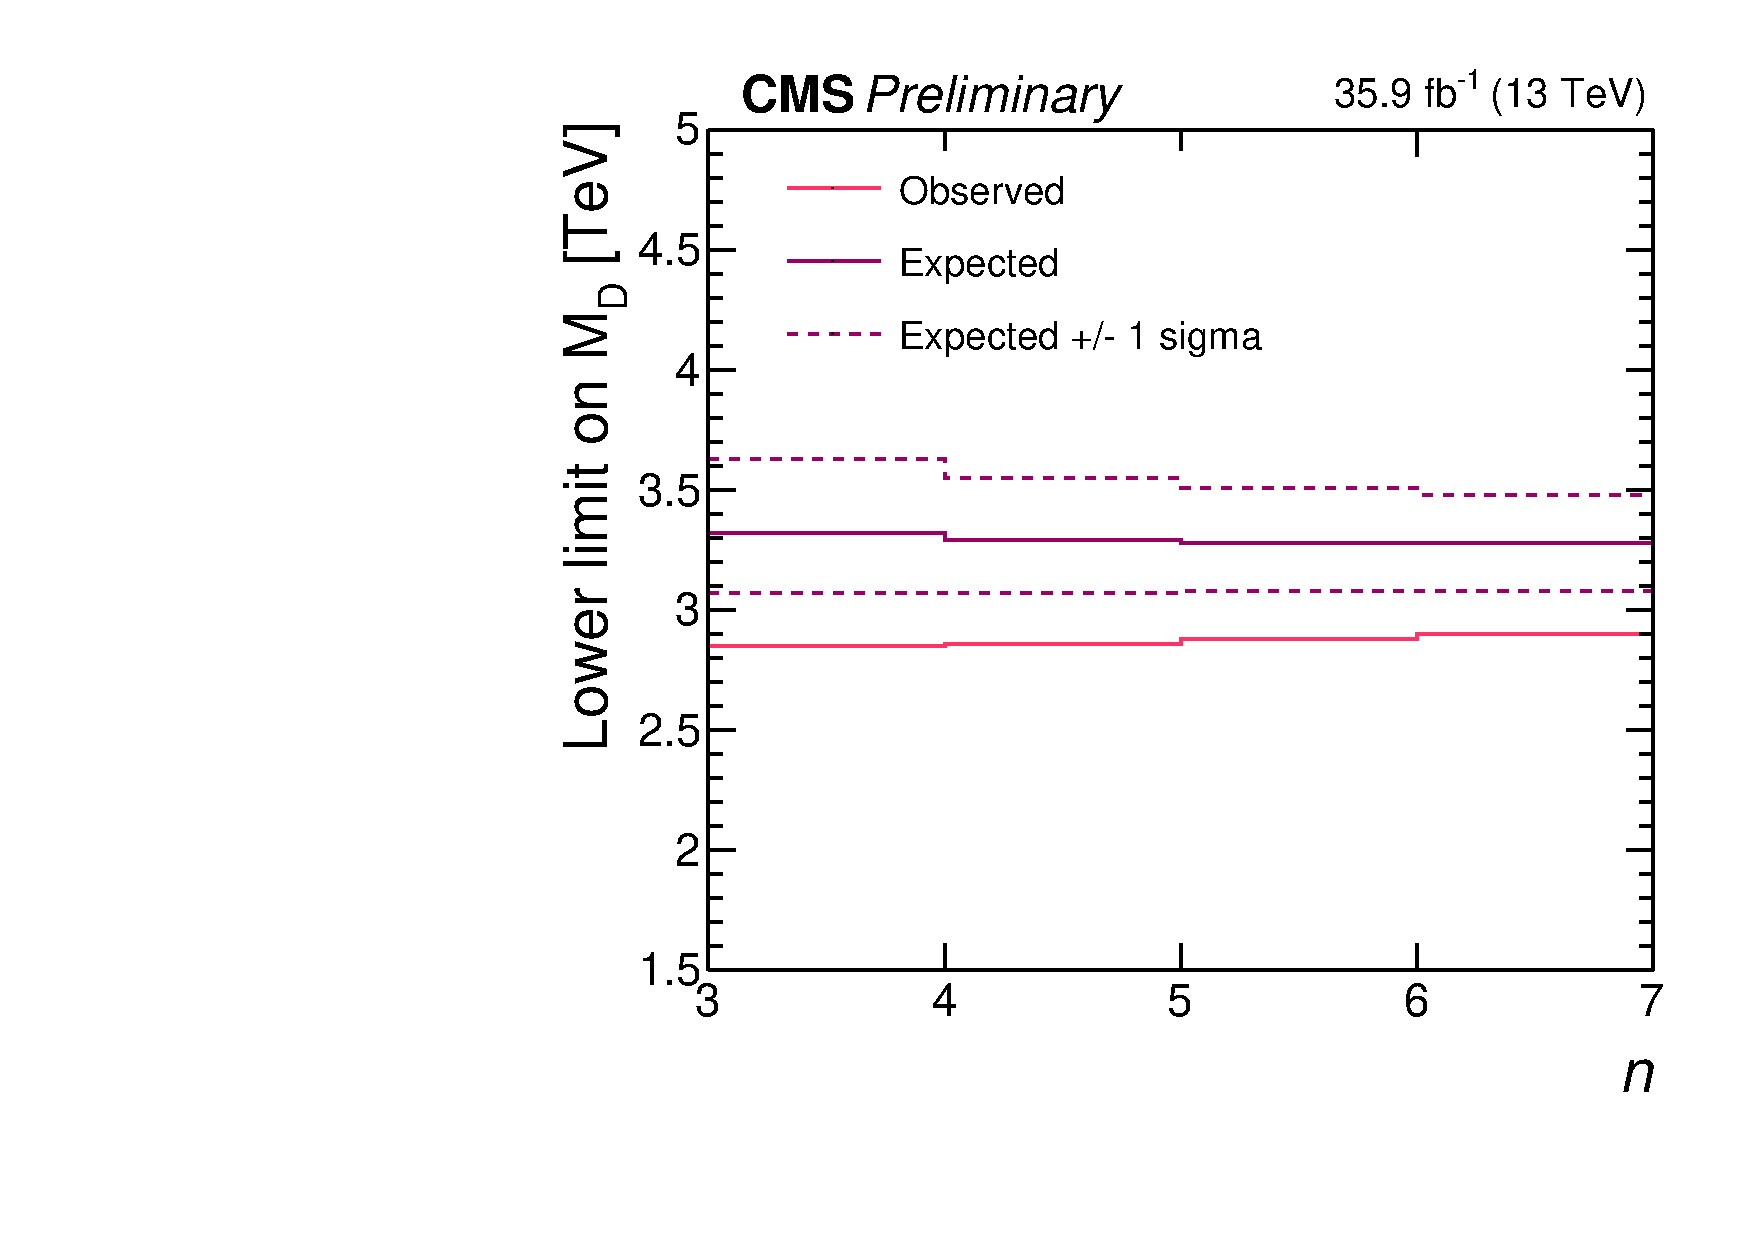
\includegraphics[width=0.5\textwidth]{figures/exo16053/Figure_011.pdf}
    \caption{The 95\% CL observed and expected lower limits on the ADD mass scale \mD\ as a function of $n$, the number of extra dimensions.
    Published in~\cite{ref:JHEP02(2019)074}.}
    \label{fig:MDLimits}
  \end{center}
\end{figure}
